\chapter{变形}\label{ch:deformation}

第九章中，我们看到可以利用粘合技术为带标记曲面构造镜像。这些范畴对应于正合流形上的 partially wrapped Fukaya 范畴。若要构造闭曲面的 Fukaya 范畴，就必须考察这些范畴的变形。本章先详细讨论 $A_\infty$ 代数的变形理论及其与 Hochschild 上同调的关系；更多细节参见\bookcite{147,153}。

随后，我们将这些概念用于带内部标记点的曲面，并讨论如何借此构造闭曲面的镜像对应。我们将考察高亏格曲面的情形，这部分工作由 Seidel\bookcite{220} 和 Efimov\bookcite{71} 完成。亏格为 $1$ 的曲线的镜像对称最初由 Polishchuk 和 Zaslow\bookcite{205} 研究，但当时只涉及普通导出范畴。包含高阶乘积的处理由 Lekili 和 Perutz\bookcite{162}、Lekili 和 Polishchuk\bookcite{164} 完成。与高亏格曲线（可以在 $\mathbb C$ 上工作）不同，椭圆曲线理论需要形式幂级数，才能使 $A_\infty$ 结构正常运作。本部分主要沿用 Cho、Hong 和 Lau\bookcite{55,154} 的工作；这一框架用途广泛，也便于向多个方向推广。

\section{\texorpdfstring{$A_\infty$}{A-infinity} 代数的变形理论}\label{sec:deformation-a-infinity}

数学的许多领域都关心对象的变形。一般地，若 $A$ 是某种定义在 $\mathbb C$ 上的对象（例如代数、模或簇），那么变形是定义在环 $\mathbb C[\hbar]/(\hbar^{n+1})$ 或 $\mathbb C[[\hbar]]$ 上的对象 $\widetilde A$，并且令变形参数 $\hbar$ 取零后可恢复 $A$。在前一种情形中，称 $\widetilde A$ 为 $n$ 阶变形；在后一种情形中，称为形式变形。以下考察 $A_\infty$ 代数或范畴的变形，并用 $\mathbb C[[\hbar]]$ 表示系数环，用 $(\hbar)$ 表示由变形参数生成的理想。
\takeaway{$A_\infty$ 代数的变形由 Hochschild 上链复形 $\mathrm{HC}^{\bullet}(A)$ 控制：一阶变形对应 $\mathrm{HH}^1(A)$，形式变形对应满足 Maurer--Cartan 方程的元素，其等价类由 $\mathrm{HC}^0$ 的指数作用给出；HKR 与 Koszul 对偶把变形理论翻译成多向量场与外代数的语言。}

\begin{definition}{$A_\infty$ 代数的变形}{ainfty-deformation}
一个 $A_\infty$ 代数 $(A,\mu)$ 的变形\index{adaishudebianxing@$A_\infty$ 代数的变形|hyperpage}，是一组乘法 $\mu+\nu$，其中
\[
  \nu_i\in\operatorname{Hom}^{1}\bigl(A[1]^{\otimes i},A[1]\bigr)\otimes(\hbar),\qquad i\geq 0,
\]
并且它们满足带曲率的 $A_\infty$ 公理。

若存在一个 $A_\infty$ 态射 $1+\phi$，其中
\[
  \phi\in\operatorname{Hom}^{0}\bigl(A[1]^{\otimes i},A[1]\bigr)\otimes(\hbar),
\]
把变形 $\mu+\nu$ 映到 $\mu+\nu'$，则称这两个变形等价。
\end{definition}

按等价分类 $A_\infty$ 代数变形的问题，可以用一种上同调理论来表述。

\begin{definition}{Hochschild 上链复形}{hochschild-cochain-complex}
$A_\infty$ 代数 $A$ 的 Hochschild 上链复形\index{hochschildshanglianfuxing@Hochschild 上链复形|hyperpage}是分次向量空间
\[
  \mathrm{HC}^{i}(A):=\prod_{k\geq0}\operatorname{Hom}_{k}^{i}\bigl(A[1]^{\otimes k},A[1]\bigr),
\]
其微分定义为
\begin{align*}
  (d\nu)_k(a_1,\ldots,a_k)
  ={}&\sum_{i,j}(-1)^{\dagger\,\deg\nu}
  \mu(a_1,\ldots,a_{i-1},\nu(a_i,\ldots,a_j),a_{j+1},\ldots,a_k)\\
  &+\sum_{i,j}(-1)^{\dagger\,\deg\mu}
  \nu(a_1,\ldots,a_{i-1},\mu(a_i,\ldots,a_j),a_{j+1},\ldots,a_k).
\end{align*}
Hochschild 复形还带有一个称为 Gerstenhaber 括号\index{gerstenhaberkuohao@Gerstenhaber 括号|hyperpage}的括号运算，使它成为微分分次 Lie 代数（dgla）：\footnote{dgla 是带有括号的上链复形，满足 $[a,b]=(-1)^{|a||b|}[b,a]$、$d[a,b]=[da,b]+(-1)^{|a|}[a,db]$ 与分次 Jacobi 恒等式。和微分分次代数类似，dgla 也有称为 $L_\infty$ 代数的 $\infty$ 推广。}
\[
\begin{aligned}
  \relax[\nu,\kappa](a_1,\ldots,a_k)
  ={}&\sum_{i,j}(-1)^{\dagger\,\deg\kappa}\,
  \nu(a_1,\ldots,a_{i-1},\\
  &\qquad\kappa(a_i,\ldots,a_j),a_{j+1},\ldots,a_k)\\
  &+\sum_{i,j}(-1)^{\dagger\,\deg\nu}\,
  \kappa(a_1,\ldots,a_{i-1},\\
  &\qquad\nu(a_i,\ldots,a_j),a_{j+1},\ldots,a_k).
\end{aligned}
\]
复形 $\mathrm{HC}^{\bullet}(A)$ 的上同调称为 Hochschild 上同调\index{hochschildshangtongdiao@Hochschild 上同调|hyperpage}，记作 $\mathrm{HH}^{\bullet}(A)$。
\end{definition}
% [Tutor Note: 定义中用直积 $\prod_{k\geq0}$ 而非直和，因此 $\mathrm{HC}^{i}(A)$ 允许同时含无穷多个不同输入个数的项；这一约定在 §12.2 的滤过与指数作用中必不可少，否则 $\exp(\phi)$ 展开出的无穷多项会越出复形。]

\begin{theorem}{$A_\infty$ 代数变形的分类}{ainfty-deformation-classification}
设 $A$ 是一个 $A_\infty$ 代数。
\begin{enumerate}[label=(\roman*)]
  \item $A$ 的一阶变形按等价分类，由 $\mathrm{HH}^{1}(A)$ 描述。
  \item $A$ 的形式变形由满足 Maurer--Cartan 方程
  \[
    \mathrm{MC}(x):=dx+\frac12[x,x]=0
  \]
  的元素 $x\in\mathrm{HC}^{1}(A)\otimes(\hbar)$ 描述。
\end{enumerate}
Maurer--Cartan 元素空间上有 Lie 代数 $\mathrm{HC}^{0}(A)\otimes(\hbar)$ 的作用：
\[
  \phi\cdot x=\partial_x\mathrm{MC}(x)(\phi)
  =d\phi+\frac12[\phi,x]+\frac12[x,\phi].
\]
该作用可积分为 Lie 群作用
\[
  \exp(\phi)\cdot x
  =x+\phi+[\phi,x]+\frac12\bigl([\phi,[\phi,x]]+[\phi,d x]\bigr)+\cdots.
\]
此作用的轨道正是变形的等价类。
\end{theorem}
\begin{proof}[证明思路]
第一条直接由定义得到。第二条可参见\bookcite{147}。
\hfill$\square$
\end{proof}

\begin{note}[约化 Hochschild 复形]
若 $A=\Bbbk 1\oplus\overline A$ 有严格单位元 $1$，可把约化 Hochschild 复形\index{yuehuahochschildfuxing@约化 Hochschild 复形|hyperpage} $\mathrm{HC}^{\bullet}_{\mathrm{red}}(A)$ 定义为 $\mathrm{HC}^{\bullet}(A)$ 的子复形，其中的 $\nu$ 只要有一个输入为 $1$ 就取零。该复形描述保持 $1$ 为严格单位元的变形。由于每个带弱单位元的 $A_\infty$ 代数都等价于一个带严格单位元的代数，可以证明 $\mathrm{HC}^{\bullet}_{\mathrm{red}}(A)$ 与 $\mathrm{HC}^{\bullet}(A)$ 拟同构。
\end{note}

\begin{example}[对偶数代数的变形]
令 $E=\mathbb C[\xi]/(\xi^2)$，其中 $\deg\xi=1$，并把它看成 $\mathbb Z_2$ 分次的 $A_\infty$ 代数。约化 Hochschild 复形中的元素由 $\nu_k(\xi,\ldots,\xi)$ 决定。若其值是 $\xi$ 的倍数，则次数为 $0$；若其值是 $1$ 的倍数，则次数为 $1$。任意取乘积
\[
  \nu_k(\xi,\ldots,\xi)=a_k\xi+b_k
\]
都会自动满足 $A_\infty$ 公理，因此微分为零。令 $a(X)=\sum_k a_kX^k$、$b(X)=\sum_k b_kX^k$，属于 $\mathbb C[[X]]$，则可作如下识别：
\[
  \mathrm{HC}^{\bullet}_{\mathrm{red}}(E)=\mathbb C[[X]]\oplus\mathbb C[[X]].
\]
复形上的括号也容易计算。若 $\nu_1$ 对应 $(X^k,0)$，而 $\nu_2$ 对应 $(0,X^\ell)$，那么可把 $\nu_k(\xi,\ldots,\xi)=\xi$ 放入 $\nu_\ell$ 的 $\ell$ 个位置中的任意一个；反过来，把 $\nu_\ell(\xi,\ldots,\xi)=0$ 放入 $\nu_k$ 则结果为零。因此 $[\nu_1,\nu_2]$ 对应于
\[
  \ell X^{k+\ell-1}=X^k\partial_X X^\ell.
\]
于是，把 $(a(X),0)$ 识别为算子 $a(X)\partial_X$，把 $(0,b(X))$ 识别为函数 $b(X)$ 是自然的。这样，$a(X)\partial_X\in\mathrm{HH}^0(E)$ 对 $b(X)\in\mathrm{HH}^1(E)$ 的作用就是通常的导数作用。

两个 $b(X)$ 型元素之间的括号为零，所以所有 $b(X)\in\mathrm{HH}^1(E)\otimes(\hbar)$ 都满足 Maurer--Cartan 方程。$\mathrm{HH}^0(E)\otimes(\hbar)$ 的导数作用积分为
\[
  \exp\bigl(a(X)\partial_X\bigr)\cdot b(X)=b\bigl(e^{a(X)}\bigr),
\]
它作用在 $\mathrm{HH}^1(E)\otimes(\hbar)$ 上。该作用的轨道对应于单项式 $\hbar^iX^j$。每种这样的变形对应一个 $A_\infty$ 结构，其中
\[
  \mu_j(\xi,\ldots,\xi)=\hbar^i,
\]
其余乘积均为零。
\end{example}
% [Tutor Note: 原文此处作 $\exp(a(X)\partial_X)\cdot b(X)=b(e^{a(X)})$；但 $\exp(a\partial_X)$ 是沿向量场 $a\partial_X$ 的时间 $1$ 流，一般给出 $X\mapsto X+a(X)+\cdots$ 的变量代换。只有当 $a(X)=cX$ 为线性时流才恰为 $X\mapsto e^{c}X=e^{a(X)}$，故一般情形下此处疑为原书笔误（见原书 p.341）；后文“轨道对应单项式”应按变量代换而非按 $e^{a}$ 理解。]

\begin{note}[dg Lie 代数与变形问题]\label{note:dgla-deformation-theory}
定理~\ref{thm:ainfty-deformation-classification} 是变形理论中的一般现象：每个变形问题都可关联一个 dgla $(L,d,[\ ,\ ])$。一阶变形由第一上同调 $H^1L$ 给出；形式变形则由 $L^1\otimes(\hbar)$ 中满足 Maurer--Cartan 方程的解给出。拟同构的 dgla 会产生同构的变形问题：形式变形的等价类与 Maurer--Cartan 解在指数化的 $L^0\otimes(\hbar)$ 作用下的轨道之间存在一一对应\bookcite{203}。

与微分分次代数的情形类似，dgla 也有极小模型的概念，这种对象称为 $L_\infty$ 代数。它带有满足适当 $L_\infty$ 公理的高阶括号 $[-,\ldots,-]$。Maurer--Cartan 方程展开为
\[
  \mathrm{MC}(x)=dx+\frac1{2!}[x,x]+\frac1{3!}[x,x,x]+\cdots=0,
\]
Lie 代数作用相应定义为 $\phi\cdot x=\partial_x\mathrm{MC}(\phi)$。有关这种变形理论方法的更多信息，可参见 Kontsevich 与 Soibelman 的在线手稿\bookcite{147}。拟同构的 $L_\infty$ 代数的 Maurer--Cartan 解等价类之间存在双射，其证明见\bookcite[附录 A]{71}。
\end{note}

\begin{note}[经典 Hochschild 上同调]
Hochschild 上同调最初只在普通的未分次代数背景下发展\bookcite{119}。由于代数 $A$ 集中在次数 $0$，空间 $\mathrm{HC}^k(A)$ 只包含 $(k+1)$ 元乘积，所以也可以按输入个数为复形分次。正因如此，在经典语境中，$\mathrm{HH}^1(A)$ 通常记作 $\mathrm{HH}^2_{\mathrm{clas}}(A)$，它描述代数的一阶变形。

经典的零阶和一阶 Hochschild 上同调也有直观解释：前者是中心，后者是外导子的空间。\footnote{经典 Hochschild 上同调的表达式采用表示论中的符号约定。这样，$m_1$ 是导子，而 $m_2$ 是普通乘法。}
\[
  \mathrm{HH}^0_{\mathrm{clas}}(A)=\{m_0\in A\mid dm_0(a)=am_0-m_0a=0\}=Z(A),
\]
\[
  \mathrm{HH}^1_{\mathrm{clas}}(A)
  =\frac{\{m_1:A\to A\mid dm_1(a,b)=m_1(ab)-m_1(a)b-am_1(b)=0\}}
  {\{dm_0:A\to A\mid a\mapsto[a,m_0]\}}
  =\frac{\operatorname{Der}(A)}{\operatorname{Inn}(A)}.
\]
经典 Hochschild 上同调还有另一种解释：把 $A$ 看成自身的双模时，它是 Ext 环；等价地，把 $A$ 看成 $A^e:=A\otimes A^{\mathrm{op}}$ 上的右模，有
\[
  \mathrm{HH}^{\bullet}_{\mathrm{clas}}(A)=\operatorname{Ext}^{\bullet}_{A^e}(A,A).
\]
这说明可以利用代数的双模分解来计算 Hochschild 上同调。
\end{note}

\begin{example}[形式幂级数环的 Hochschild 上同调]
令 $A=\mathbb C[[X]]$，则它有如下双模分解：
\[
  B^{\bullet}:=A\otimes A\xrightarrow{\,X\otimes1-1\otimes X\,}A\otimes A.
\]
复形 $\operatorname{Hom}_{A^e}(B^{\bullet},A)$ 为 $A\xrightarrow{0}A$，所以
\[
  \mathrm{HH}^{\bullet}_{\mathrm{clas}}(A)=A\oplus A.
\]
经典零阶上同调是中心 $A$，一阶上同调是由 $A\partial_X$ 给出的导子。恢复 $A_\infty$ 分次后，
\[
  \mathrm{HH}^{\bullet}(A)=A\partial_X\oplus A,
\]
因此 $A=\mathbb C[[X]]$ 的 Hochschild 上同调实际上与例~12.5 中 $E=\mathbb C[\xi]/(\xi^2)$ 的相同。不过，此处变形 $\hbar^iX^j$ 有不同解释：它把 $\mathbb C[[X]]$ 变形成带曲率的 $A_\infty$ 代数 $(\mathbb C[[X]],\hbar^iX^j)$。

上述例子可以推广到箭图。令 $A=\widehat{\mathbb C Q}/I$ 为完备路径代数，关系由长度为 $2$ 的路径生成。令 $Z_0=Q_0$、$Z_1=Q_1$；对 $n\geq2$，令 $Z_n$ 为所有路径 $a_1\cdots a_n$ 的集合，其中每个长度至少为 $2$ 的子路径（包括路径本身）都属于 $I$。对每条路径 $p$，定义双模
\[
  B[p]=A_{h(p)}\otimes[p]\otimes_{t(p)}A,
\]
并以 $[p]$ 记其生成元。现在令
\[
  B_i=\bigoplus_{a_1\cdots a_n\in Z_i}B[a_1\cdots a_n],
\]
微分定义为
\[
  d[a_1\cdots a_n]=a_1[a_2\cdots a_n]-(-1)^k[a_1\cdots a_{n-1}]a_n.
\]
\end{example}

\begin{theorem}{Bardzell 双模分解}{bardzell-resolution}
复形 $B^{\bullet}$ 是 $A$ 的投射双模分解，因此
\[
  \mathrm{HH}^{\bullet}_{\mathrm{clas}}(A)\cong H\operatorname{Hom}^{\bullet}_{A^e}(B^{\bullet},A).
\]
\end{theorem}
\begin{proof}[证明思路]
容易验证 $B[p]$ 是投射模且 $d^2=0$。此外，在 $H B_0$ 中，表达式 $p[h(a)]a q$ 与 $p a[t(a)]q$ 相同，所以可以把所有因子移到左边，从而 $H B_0=\bigoplus_{v\in Q_0}A_v=A$。其余同调为零的证明见\bookcite{21}。
\hfill$\square$
\end{proof}

\begin{example}[循环箭图的 Hochschild 上同调]
考虑顶点为 $v_i$、箭头为 $a_i:v_i\leftarrow v_{i+1}$ 的循环箭图，其中 $i\in\mathbb Z_n$ 且 $n\geq2$。先考虑没有关系的箭图。此时当 $n\geq2$ 时 $Z_n=\varnothing$，因此分解只有两项：
\[
  \bigoplus_{v\in Q_0}A_v[v]_vA\xleftarrow{\ a[t(a)]-[h(a)]a\ }\bigoplus_{a\in Q_1}A_{h(a)}[a]_{t(a)}A.
\]
由此得到
\[
  \mathrm{HH}^0_{\mathrm{clas}}(A)=Z(A)=\mathbb C[\ell],\qquad
  \mathrm{HH}^1_{\mathrm{clas}}(A)=\mathbb C[\ell]\delta,\qquad
  \mathrm{HH}^{>2}_{\mathrm{clas}}(A)=0,
\]
其中
\[
  \ell=a_1\cdots a_n+\cdots+a_n\cdots a_{n-1},\qquad \delta([a_i])=a_i.
\]

再考察对偶箭图代数 $E=\Lambda_Q=\operatorname{Ext}^{\bullet}(S,S)$，其中 $S$ 是顶点简单模的直和。可将 $E$ 写成顶点为 $v_i$、箭头为 $\alpha_i:v_{i+1}\leftarrow v_i$，关系为 $\alpha_{i+1}\alpha_i=0$ 的路径代数。此时 $Z_k$ 由所有长度为 $k$ 的路径组成。由于 $\Lambda_Q$ 中只有顶点和箭头对应非零路径，只有当 $k\equiv0,1\pmod n$ 时，才可能存在态射 $B_k\to E$。

\begin{itemize}
  \item 若 $k=rn$，双模态射 $f:B_k\to E$ 由常数 $\lambda_i$ 确定，使得
  \[
    f([\alpha_{i+rn-1}\cdots\alpha_i])=\lambda_i v_i.
  \]
  条件 $df=0$ 蕴含所有 $\lambda_i$ 相等，而 $\operatorname{Hom}_{E^e}(B_{rk},E)$ 中 $d$ 的像为零。因此
  \[
    \mathrm{HH}^{rn}_{\mathrm{clas}}(E)
    =\mathbb C\left(\sum_i[\alpha_{i+rn-1}\cdots\alpha_i\to v_i]\right)=:\mathbb C\Omega_{r,0}.
  \]
  \item 若 $k=rn+1$，双模态射 $f:B_k\to E$ 由常数 $\lambda_i$ 确定，使得
  \[
    f([\alpha_{i+rn}\cdots\alpha_i])=\lambda_i\alpha_i.
  \]
  此时 $df=0$ 自动成立，而
  \[
    d[\alpha_{i+rn-1}\cdots\alpha_i\to v_i]
    =[\alpha_{i+rn}\cdots\alpha_i\to\alpha_i]
    -[\alpha_{i+rn}\cdots\alpha_i\to\alpha_i],
  \]
  所以在等价意义下可令所有 $\lambda_i$ 相等：
  \[
    \mathrm{HH}^{rn+1}_{\mathrm{clas}}(E)
    =\mathbb C\left(\sum_i[\alpha_{i+rn}\cdots\alpha_i\to\alpha_i]\right)=:\mathbb C\Omega_{r,1}.
  \]
\end{itemize}
若将 $\ell^j1$ 对应于 $\Omega_{r,0}$，将 $\ell^i\delta$ 对应于 $\Omega_{r,1}$，则在 $A_\infty$ 分次下，$A$ 与 $E$ 的 Hochschild 上同调之间有对应
\[
  \mathrm{HH}^{0}(A)=\mathbb C[[\ell]]\delta=\mathrm{HH}^{0}(E),\qquad
  \mathrm{HH}^{-1}(A)=\mathbb C[[\ell]]=\mathrm{HH}^{-1}(E).
\]
在这一分次下，所有 $\Omega_{r,0}$ 的次数为 $-1$，所有 $\Omega_{r,1}$ 的次数为 $0$。该对应也与 Gerstenhaber 括号所给的额外结构相容：两边都有
\[
  [\ell^i\delta,\ell^j]=n j\ell^{i+j},
\]
所以 $\ell^i\delta\in\mathrm{HH}^{0}(A)$ 对 $\mathrm{HH}^{0}(E)$ 的作用是导数 $n\ell^{i+1}\partial_\ell$。与例~12.5 类似，这说明每个变形都等价于由一个单项式给出的变形，进而得到 Landau--Ginzburg 模型 $(\widehat{\mathbb C Q},\hbar\ell^j)$ 与 $A_\infty$ 代数 $(E,\mu_{\hbar,j})$ 之间的对应；后者唯一非零的乘积为
\[
  \mu_{\hbar,j}(\alpha_i,\ldots,\alpha_{i+jn-1})=\hbar h(\alpha_i).
\]
% [Tutor Note: 原文写 $\ell^i\delta\in\mathrm{HH}^{0}(A)$ 作用在 $\mathrm{HH}^{0}(E)$ 上；但按前述分次，$\ell^j$ 位于 $\mathrm{HH}^{-1}$，而括号给出 $[\ell^i\delta,\ell^j]=nj\ell^{i+j}\in\mathrm{HH}^{-1}$，故作用对象疑应为 $\mathrm{HH}^{-1}(E)$（原书 p.344），此处沿原文保留。]

这属于称为 Koszul 对偶\index{koszulduiou@Koszul 对偶|hyperpage}的一般现象。任意完备路径代数 $A=\widehat{\mathbb C Q}/I$ 及其 Koszul 对偶 $A_\infty$ 代数 $\operatorname{Ext}^{\bullet}_A(S,S)$ 的 Hochschild 复形都是 $L_\infty$ 拟同构的\bookcite{134}。第~\ref{sec:koszul-duality} 节将更详细讨论这一现象。
\end{example}

Hochschild 上同调在其他一些构造下也保持不变。不过，在进一步讨论之前，需要先把 Hochschild 上同调的概念推广到 $A_\infty$ 范畴。推广并不困难：若 $\mathcal A^{\bullet}$ 是 $A_\infty$ 范畴，令
\[
  \mathrm{HC}^{i}(\mathcal A^{\bullet})
  :=\prod_{k\geq0}\prod_{X_0,\ldots,X_k\in\mathcal A^{\bullet}}
  \operatorname{Hom}^{i}_{\mathbb C}\bigl(
  \mathcal A^{\bullet}(X_{k-1},X_k)\otimes\cdots\otimes
  \mathcal A^{\bullet}(X_0,X_1),\mathcal A^{\bullet}(X_0,X_k)\bigr),
\]
并按代数情形相同的方式定义微分与括号。

\begin{theorem}{Hochschild 复形的不变性}{hochschild-invariance}
以下相关的 $A_\infty$ 代数与范畴具有拟同构的 Hochschild 复形：
\begin{enumerate}[label=(\roman*)]
  \item 拟 $A_\infty$ 等价的 $A_\infty$ 范畴；
  \item 一个 $A_\infty$ 范畴及其扭曲完备化；
  \item （分裂）导出等价的 $A_\infty$ 范畴；
  \item $A=\widehat{\mathbb C Q}/I$ 与 $E=\operatorname{Ext}^{\bullet}_A(S,S)$，其中 $S=A/\langle a\in Q_1\rangle$。
\end{enumerate}
\end{theorem}
\begin{proof}[证明思路]
这些结论在微分分次代数的语境中早已为人所知，而该语境与 $A_\infty$ 语境等价。不同一般性层次的证明可见多种文献。例如，文献\bookcite{134} 证明了这些拟同构还与 Gerstenhaber 括号给出的 $L_\infty$ 结构等额外结构相容。
\hfill$\square$
\end{proof}

\begin{example}[多项式环的 Hochschild--Kostant--Rosenberg 对应]
令 $\widehat R=\mathbb C[[X_1,\ldots,X_n]]$ 为集中在次数 $0$ 的完备多项式环，令 $\Lambda=\operatorname{Ext}^{\bullet}_{\widehat R}(S,S)$ 为由对偶变量 $\xi_1,\ldots,\xi_n$ 生成、每个变量次数为 $1$ 的外代数。每个 $\xi_i$ 可视为 $\widehat R$ 上的导数 $\partial_{X_i}$，乘积 $g(X)\xi_{i_1}\cdots\xi_{i_k}$ 可解释为映射 $\nu_k:\widehat R^{\otimes k}\to\widehat R$：
\[
  \nu_k(f_1(X),\ldots,f_k(X))
  =g(X)\sum_{\sigma\in S_k}\frac{(-1)^\sigma}{k!}
  \partial_{X_{i_{\sigma(1)}}}f_1(X)\cdots
  \partial_{X_{i_{\sigma(k)}}}f_k(X).
\]
由此得到映射
\[
  F:\widehat R\otimes\Lambda\longrightarrow\mathrm{HH}^{\bullet}_{\mathrm{clas}}(\widehat R).
\]
著名的 Hochschild--Kostant--Rosenberg 定理\index{hochschildkostantrosenbergdingli@Hochschild–Kostant–Rosenberg 定理|hyperpage}\bookcite{116} 说明 $F$ 是分次向量空间的同构。

在 $\widehat R\otimes\Lambda$ 上令 $d=0$，并规定
\[
  [X_i,\xi_j]=\delta_{ij},\qquad [X_i,X_j]=[\xi_i,\xi_j]=0,
\]
再通过分次 Poisson 规则
\[
  [a,bc]=[a,b]c+(-1)^{\deg b(\deg a-1)}[b,ac]
\]
把括号延拓至整个 $\widehat R\otimes\Lambda$，即可赋予其 dgla 结构。按原分次，括号的次数为 $-1$；对 $\widehat R\otimes\Lambda[1]$ 而言，括号的次数为 $0$。

Kontsevich 同样著名的形式性定理\index{kontsevichxingshixingdingli@Kontsevich 形式性定理|hyperpage}\bookcite{143,242} 断言，$F$ 可延拓为一个 $L_\infty$ 同构
\[
  F_{\bullet}:\widehat R\otimes\Lambda[1]\longrightarrow\mathrm{HH}(\widehat R).
\]
此时 $\widehat R\otimes\Lambda[1]$ 上的 Maurer--Cartan 方程化为 $[\psi,\psi]=0$，其中
\[
  \psi\in\widehat R\otimes\Lambda[1]^1\otimes(\hbar)
  =\widehat R\otimes\Lambda^2\otimes(\hbar).
\]
满足该方程的解称为 Poisson 双向量。形式性定理蕴含每个 Poisson 双向量都对应于 $\widehat R$ 的一个形式变形。

若采用 $\mathbb Z_2$ 分次，也可以考虑与每个偶数次的 $\widehat R\otimes\Lambda^k\otimes(\hbar)$ 元素相对应的变形。特别地，$f(X)\in\widehat R\otimes\Lambda^0\otimes(\hbar)$ 自动满足 $[f,f]=0$，并对应一个 Landau--Ginzburg 模型 $(\widehat R,f)$，即 $\widehat R$ 的带曲率变形。

要判断两个这样的带曲率变形是否等价，需要考察 $\mathrm{HH}^{0}(\widehat R)=\mathrm{HH}^{\mathrm{odd}}_{\mathrm{clas}}(\widehat R)$ 的作用。这样的元素形如 $\sum_i g_i(X)\xi_i+K$，其中 $K$ 含有 $\xi_i$ 的高次项。若将它与函数 $f(X)$ 作括号，则
\[
  \left[\sum_i g_i(X)\xi_i+K,f(X)\right]
  =\sum_i g_i(X)\partial_{X_i}f(X)+[K,f(X)].
\]
第二项仍含有 $\xi_i$ 的幂，因此若要留在函数构成的子空间内，必须要求 $K=0$。元素 $\sum_i g_i(X)\xi_i$ 对 $\widehat R$ 的作用是导数作用；而 $\widehat R=\mathrm{HH}^{0}_{\mathrm{clas}}(\widehat R)\subset\mathrm{HH}^{1}(\widehat R)$，将此作用积分后便得到 $\operatorname{Aut}(\widehat R)$ 的作用。因此，两个带曲率变形 $f,f'$ 等价，当且仅当它们属于同一个 $\operatorname{Aut}(\widehat R)$ 轨道。
\end{example}

\begin{example}[由矩阵分解得到的变形]
前一例也可从外代数的角度处理。由 Koszul 对偶，$\mathrm{HH}^{\bullet}(\widehat R)$ 与 $\mathrm{HH}^{\bullet}(\Lambda)$ 等价，因此可以把 $\widehat R$ 的变形传递为 $\Lambda$ 的变形。

考虑微分形式环
\[
  \Omega=\widehat R\langle dX_1,\ldots,dX_n\rangle,
\]
把它看成 $\mathbb Z_2$ 分次的 $\widehat R$ 模，并令 $\delta\omega=\iota_\eta\omega$，其中 $\eta=\sum_i X_i\partial_i$。这样得到的扭曲复形 $(\Omega,\delta)$ 可看作 $S$ 的一个分解。于是
\[
  E:=\bigl(\operatorname{Hom}_{\widehat R}(\Omega,\Omega),[\delta,-]\bigr)
\]
是 $\Lambda$ 的一个 dg 模型。

若把 $\widehat R$ 变形为 Landau--Ginzburg 模型 $(\widehat R,\hbar f)$，其中 $f\in(X)$，则 dg 代数 $E$ 变形为带曲率 dg 代数
\[
  E_f=(E,\hbar f\,1_\Omega).
\]
另一方面，如第~\ref{subsec:matrix-factorizations-projective-varieties} 节所述，也可以把 $(\Omega,\delta)$ 变形为 $f$ 的矩阵分解。写成 $f=X_1f_1+\cdots+X_nf_n$，并令 $\gamma=f_1dX_1+\cdots+f_ndX_n$，则 $\iota_\eta(\gamma)=f$，且对任意 $\omega\in\Omega$，
\begin{align*}
  (\delta+\hbar\gamma\wedge)^2\omega
  &=\iota_\eta\iota_\eta\omega+\iota_\eta(\hbar\gamma\wedge\omega)
    +\hbar\gamma\wedge\iota_\eta\omega+\hbar^2\gamma\wedge\gamma\wedge\omega\\
  &=0+\iota_\eta(\hbar\gamma)\wedge\omega+0
   =\hbar f\omega.
\end{align*}
矩阵分解 $(\Omega,\delta+\hbar\gamma\wedge)$ 的自同态环
\[
  E_\gamma=\bigl(\operatorname{Hom}_{\widehat R}(\Omega,\Omega),[\delta+\hbar\gamma\wedge,-]\bigr)
\]
是 $E$ 的一个变形。变形 $E_\gamma$ 与 $E_f$ 在 Hochschild 上同调中由同一个元素 $f=[\gamma\wedge,-]\in\mathrm{HC}^{1}(E)$ 表示，因为若把 $\gamma\wedge$ 看成
\[
  \operatorname{Hom}^{1}(\Omega,\Omega)=E[1]^0
  =\operatorname{Hom}^{0}_{\mathbb C}(E[1]^{\otimes0},E[1])\subset\mathrm{HC}^{0}(E),
\]
则
\[
  d_{\mathrm{HC}}(\gamma\wedge)=\delta\gamma-[\gamma\wedge,-]=f-[\gamma\wedge,-].
\]
\end{example}

\begin{note}[Hochschild--Kostant--Rosenberg 定理]\index{hochschildkostantrosenbergdingli@Hochschild–Kostant–Rosenberg 定理|hyperpage}
一般而言，Hochschild--Kostant--Rosenberg 定理说明光滑仿射簇 $X$ 的 Hochschild 上同调等于其多向量场环。从代数角度看，若 $R$ 是 $X$ 的坐标环，则
\[
  \mathrm{HH}^{\bullet}_{\mathrm{clas}}(R)=\Lambda_R^{\bullet}\operatorname{Der}_R.
\]
对非仿射簇也可以作类似构造，不过此时多向量场环是定义在结构层 $\mathcal O_X$ 上的环层，而 Hochschild 上同调则是该层的上同调。
\end{note}

\section{\texorpdfstring{$A_\infty$}{A-infinity} 扩张}\label{sec:ainfty-extensions}

Hochschild 上同调不仅适用于研究 $A_\infty$ 代数的无穷小变形，也是研究一个相关问题的便利工具。
\takeaway{固定底层分次代数后，$A_\infty$ 扩张的等价类由滤过 $\mathrm{HC}^1(A)$ 中满足 Maurer--Cartan 方程的元素控制，等价关系来自滤过 $\mathrm{HC}^0(A)$ 的指数作用；Efimov 定理说明这类扩张能把 Landau--Ginzburg 模型重构到变量代换的程度。}

\begin{definition}{$A_\infty$ 扩张}{ainfty-extension}
设 $(A,\cdot)$ 是分次代数。$A$ 上的一个 $A_\infty$ 结构，或称 $A$ 的一个 $A_\infty$ 扩张\index{akuozhang@$A_\infty$ 扩张|hyperpage}，是一组乘积 $\mu_i:A^{\otimes i}\to A$，满足 $A_\infty$ 公理，且
\[
  \mu_0=\mu_1=0,\qquad \mu_2(a,b)=(-1)^{\deg a}a\cdot b.
\]
若存在 $A_\infty$ 函子 $F:(A,\mu)\to(A,\nu)$ 且 $F_1=1_A$，则称两个 $A_\infty$ 结构 $\mu,\nu$ 等价。若 $A$ 上的一个 $A_\infty$ 结构等价于满足 $\mu_{\geq3}=0$ 的结构，则称它是平凡的。
\end{definition}

$A$ 的 Hochschild 复形带有如下滤过：
\[
  F_r\mathrm{HC}^{i}(A)
  :=\prod_{k\geq r+i+1}\operatorname{Hom}^{i}_{\mathbb C}\bigl(A[1]^{\otimes k},A[1]\bigr),
\]
并满足
\[
  dF_r\mathrm{HC}^{i}(A)\subset F_r\mathrm{HC}^{i+1}(A),\qquad
  [F_r\mathrm{HC}^{i}(A),F_s\mathrm{HC}^{j}(A)]
  \subset F_{r+s}\mathrm{HC}^{i+j}(A).
\]
$A$ 上的 $A_\infty$ 结构可视为 $\mu\in F_1\mathrm{HC}^{1}(A)$ 中满足 Maurer--Cartan 方程的元素；两个 $A_\infty$ 结构等价，当且仅当它们由某个 $\exp(\phi)$ 的作用相连，其中 $\phi\in F_1\mathrm{HC}^{0}(A)$。由于 $\exp(\phi)\cdot\mu$ 中相继各项在滤过中的阶数不断提高，此作用是有意义的。注意 $\mathrm{HC}^0(A)$ 与 $\mathrm{HC}^1(A)$ 也含有滤过次数为零或负数的部分；这些部分必须排除，否则 Maurer--Cartan 方程或指数作用可能不收敛。

\begin{note}[滤过的 $L_\infty$ 代数]
可以发展滤过 $L_\infty$ 代数的概念，并考察 Maurer--Cartan 元素在等价关系下的分类。与第~\ref{note:dgla-deformation-theory}~节的注类似，滤过 $L_\infty$ 代数的拟同构会导出 Maurer--Cartan 元素等价类之间的双射\bookcite[附录 A]{71}。
\end{note}

\begin{example}[由函数变形诱导的外代数扩张]
令 $\widehat R=\mathbb C[[X_1,\ldots,X_n]]$，令 $\Lambda$ 为由对偶变量 $\xi_1,\ldots,\xi_n$ 生成、每个变量次数为 $1$ 的外代数。取 $f\in(X)^3$，并考虑 Landau--Ginzburg 模型 $(\widehat R,f)$ 的矩阵分解 $(\Omega,\delta+\gamma\wedge)$。由于 $f$ 不含线性项，该矩阵分解的自同态环，其极小模型作为向量空间同构于 $\Lambda$；又因为 $f$ 不含二次项，其乘法结构也与 $\Lambda$ 相同。$f$ 的高次项会在 $\Lambda$ 上诱导一个 $A_\infty$ 结构，记作 $\Lambda_\gamma$。按照前述滤过，可以把 $f\in(X)^k$ 看成 $F_{k-2}\mathrm{HH}^1(\Lambda)$ 中的元素。

Efimov 在文献\bookcite[第 8 节]{71} 中证明，$\Lambda_\gamma$ 的等价类可以在变量代换的意义下重构 $f$。
\end{example}

\begin{theorem}{Efimov}{efimov-a-infinity-extensions}
设 $f_1,f_2\in(X)^3$，并分别选择 $\gamma_1,\gamma_2$，从 Landau--Ginzburg 模型
\[
  (\Omega,\delta+\gamma_i\wedge)\in\mathrm{MF}^{\pm}(\widehat R,f_i)
\]
构造自同态环 $\Lambda_{\gamma_i}$。若存在 $A_\infty$ 同构 $F_{\bullet}:\Lambda_{\gamma_1}\to\Lambda_{\gamma_2}$ 且 $F_1=1_\Lambda$，则存在变量代换 $X_i\mapsto X_i+O_i$，其中 $O_i\in(X)^2$，把 $f_1$ 变为 $f_2$。
\end{theorem}

\section{温和代数的变形理论}\label{sec:gentle-algebra-deformations}

设 $(S,M)$ 是一个闭的带标记曲面，亏格为 $g$，且有 $n$ 个内部标记点。取一组剖分 $(S,M)$ 的弧系 $A$，令 $Q$ 为其底层温和 $A_\infty$ 代数 $\mathrm{Gtl}^{\pm}A$ 的箭图。以 $F$ 表示 $A$ 中的多边形（或面）的集合。由 Euler 示性数可得
\[
  |Q_0|=|A|=2g-2+|M|+|F|=2g-2+n+|F|,
\]
而 $|Q_1|=2|Q_0|$，因为每个顶点（弧）有两个入箭（角）。每个箭头 $\alpha$ 恰好绕某个标记点和某个面各一周。对 $i\in M\cup F$，记绕 $i$ 的角的数目为 $n_i$。
\takeaway{温和代数 $A$ 的 Hochschild 上同调由绕标记点的中心元 $\ell_m$ 与绕面的元素 $\ell_f^r$ 显式给出；这些类参数化 $\mathrm{HH}^1$ 中的 Maurer--Cartan 元素，从而把温和 $A_\infty$ 结构刻画为面处高阶乘积非零的 $A_\infty$ 扩张。}

令 $A$ 表示温和 $A_\infty$ 代数 $\mathrm{Gtl}^{\pm}A$ 的底层 $\mathbb Z_2$ 分次代数。它是带二次关系的箭图路径代数，因此可以用 Bardzell 的双模分解计算 $A$ 的 Hochschild 上同调。

\begin{itemize}
  \item 对每个 $m\in M$，取所有绕 $m$ 的箭头 $\alpha_1,\ldots,\alpha_{n_m}$，构造中心元素
  \[
    \ell_m=\alpha_{n_m}\cdots\alpha_1+\cdots+\alpha_1\alpha_{n_m}\cdots\alpha_2\in Z(A),
  \]
  并构造导子
  \[
    \partial_m:A\to A,\qquad
    \alpha\longmapsto\begin{cases}
      \alpha,&\alpha\in\{\alpha_1,\ldots,\alpha_{n_m}\},\\
      0,&\text{其他情形}.
    \end{cases}
  \]
  \item 对每个 $f\in F$ 及 $r\geq1$，取所有绕 $f$ 的箭头 $\alpha_1,\ldots,\alpha_{n_f}$，仿照例~12.10 构造映射
  \[
    \ell_f^r:=\sum_{i=1}^{n_f}[\alpha_{i+rn_f-1}\cdots\alpha_i\to t(\alpha_i)]
      \in\mathrm{HH}^{rn_f}_{\mathrm{clas}}(A),
  \]
  \[
    \ell_f^r\partial_f:=\sum_{i=1}^{n_f}[\alpha_{i+rn_f}\cdots\alpha_i\to\alpha_i]
      \in\mathrm{HH}^{rn_f+1}_{\mathrm{clas}}(A).
  \]
\end{itemize}

\begin{theorem}{温和代数的经典 Hochschild 上同调}{gentle-classical-hochschild}
代数 $A$ 的经典 Hochschild 上同调具有如下结构：
\begin{align*}
  \mathrm{HH}^{0}_{\mathrm{clas}}(A)
  &\cong\mathbb C\oplus\bigoplus_{m\in M,\,r\geq1}\mathbb C\ell_m^r,\\
  \mathrm{HH}^{1}_{\mathrm{clas}}(A)
  &\cong\mathbb C^{|Q_0|+1}\oplus\bigoplus_{m\in M,\,r\geq1}\mathbb C\ell_m^r\partial_{\ell_m},\\
  \bigoplus_{k\geq2}\mathrm{HH}^{k}_{\mathrm{clas}}(A)
  &\cong\bigoplus_{f\in F,\,r\geq1}\mathbb C\ell_f^r
    \oplus\mathbb C\ell_f^r\partial_f.
\end{align*}
\end{theorem}
\begin{proof}[证明思路]
零阶和一阶 Hochschild 上同调都可以直接求出。对零阶而言，可验证每个中心元素都是 $\ell_m$ 的幂的线性组合，并且当 $m\ne m'$ 时 $\ell_m\ell_{m'}=0$。

一阶 Hochschild 上同调是外导子的空间。导子由其在每个箭头上的取值确定。若箭头 $\alpha_i$ 绕标记点 $m$，则可以把 $\alpha_i$ 映到 $f(\ell_m)\alpha_i$。可以证明，这就是 $A$ 上全部可能的导子。

若弧（顶点）$a$ 与 $m$ 相连，则由与 $\ell_m^i1_a$ 作交换所给出的内导子，会把终点为 $a$ 的角箭头 $\alpha_u$ 映到 $\ell_m^i\alpha_u$，并把起点为 $a$ 的箭头 $\alpha_{u+1}$ 映到 $-\ell_m^i\alpha_{u+1}$。当 $i>0$ 时，其他标记点周围的所有箭头都映到零。因此，模去内导子后，可以假定 $m$ 周围的所有 $\alpha_i$ 都乘以同一个非恒定因子 $\lambda_{m,i}\ell_m^i$。

对常数因子而言，与 $1_a$ 作交换会把到达 $a$ 的两个角箭头乘以 $1$，把离开 $a$ 的箭头乘以 $-1$。因此，次数为 $0$ 的外导子空间维数为
\[
  |Q_1|-(|Q_0|-1)=|A|+1,
\]
其中加上的 $1$ 来自与恒等元 $1=\sum_a1_a$ 作交换所得的平凡导子。

高阶 Hochschild 上同调可用 Bardzell 的双模分解计算。注意 $B_{\geq1}$ 按 $B[p]$ 所对应路径 $p$ 所在的多边形分解为直和，所以计算基本上与例~12.10 相同。更多细节见\bookcite{1,36}。
\hfill$\square$
\end{proof}

要把上述结果转到 $A_\infty$ 语境中，必须谨慎。在 $\mathbb Z_2$ 分次下，$\ell_m^r$ 与 $\ell_f^r$ 的 $A_\infty$ 次数都是 $1$，所以它们构成 $\mathrm{HH}^1(A)$ 的部分。不过，后者分别处于不同的经典次数，而 $\mathrm{HH}^{\bullet}(A)=\prod_i\mathrm{HH}^i(A)$，因此可以对 $\ell_f$ 作形式求和，却不能对 $\ell_m$ 作形式求和。于是
\[
  \mathrm{HH}^{0}(A)
  =\bigoplus_{m\in M}\mathbb C[\ell_m]\ell_m\partial_m
   \oplus\bigoplus_{f\in F}\mathbb C[[\ell_f]]\ell_f\partial_f
   \oplus\mathbb C^{|A|+1},
\]
\[
  \mathrm{HH}^{1}(A)
  =\frac{\mathbb C[\ell_m\mid m\in M][[\ell_f\mid f\in F]]}
  {(\ell_i\ell_j\mid i\ne j,\ i,j\in F\cup M)}.
\]
采用这种记号，是为了使 $[\ell_i^j\partial_{\ell_i},-]$ 对 $\mathrm{HH}^1(A)$ 的作用恰好成为导数 $\ell_i^j\partial_i$。
% [Tutor Note: $C[\ell_m]$ 与 $C[[\ell_f]]$ 的不对称来自 $\mathrm{HH}^{\bullet}(A)=\prod_i\mathrm{HH}^{i}(A)$ 是直积：$\ell_f$ 的各次幂落在不同的经典次数里，故允许作形式幂级数；而 $\ell_m$ 的各次幂落在同一经典次数中，取无穷和会越出直和，只能保留有限线性组合。]

\begin{note}[形式完备化]
通过转向形式完备化 $\widehat A$，可以恢复 $\ell_m$ 与 $\ell_f$ 之间的不对称性。这样，所有 $\ell_i$ 都成为形式变量。
\end{note}

温和 $A_\infty$ 代数是底层代数 $A$ 的一个 $A_\infty$ 扩张。利用 $A$ 的 Hochschild 上同调，可以得到一个简洁判据，用来检验给定的 $A_\infty$ 扩张是否同构于温和代数。

\begin{theorem}{温和 $A_\infty$ 结构的判据}{gentle-ainfty-classification}
设 $A$ 的一个 $A_\infty$ 扩张满足：对每个面 $f\in F$，绕该面的一组高阶乘积均非零，即存在 $\lambda_f\in\mathbb C\setminus\{0\}$，使得对每个 $i$，
\[
  \mu_{n_f}(\alpha_{i+n_f-1},\ldots,\alpha_i)=\lambda_f t(\alpha_i).
\]
那么此 $A_\infty$ 扩张与 $\mathrm{Gtl}^{\pm}A$ 的 $A_\infty$ 结构同构。
\end{theorem}
\begin{proof}[证明思路]
这样的扩张对应于一个 Maurer--Cartan 元素
\[
  \sum_{f\in F}\lambda_f\ell_f+\text{高阶项}.
\]
作用 $\ell_f^j\partial_f$ 积分后给出变量代换 $\ell_f\mapsto\ell_f+O(\ell_f)$，可用它消去高阶项。角态射作缩放，则可把所有 $\lambda_f$ 归一化为 $1$。更多细节见\bookcite{36}。
\hfill$\square$
\end{proof}

\begin{theorem}{温和 $A_\infty$ 代数的 Hochschild 上同调}{gentle-ainfty-hochschild}
温和 $A_\infty$ 代数 $\mathrm{Gtl}^{\pm}A$ 的 Hochschild 上同调为
\[
  \mathrm{HH}^{0}(\mathrm{Gtl}^{\pm}A)
  =\bigoplus_{m\in M}\mathbb C[\ell_m]\ell_m\partial_m\oplus\mathbb C^{n+2g-1},
\]
\[
  \mathrm{HH}^{1}(\mathrm{Gtl}^{\pm}A)
  =\frac{\mathbb C[\ell_m\mid m\in M]}
  {(\ell_i\ell_j\mid i\ne j,\ i,j\in M)}.
\]
\end{theorem}
\begin{proof}[证明思路]
作为分次向量空间，$A$ 与 $\mathrm{Gtl}^{\pm}A$ 的 Hochschild 复形相同，但微分不同：
\[
  d_{\mathrm{Gtl}^{\pm}A}=d_A+[\mu_{\geq3},-].
\]
利用谱序列\bookcite{253}，可将 $d_A$ 的上同调与 $d_{\mathrm{Gtl}^{\pm}A}$ 的上同调联系起来。后者成为复形 $(\mathrm{HH}(A),[\sum_f\ell_f, -])$ 的上同调。对每个面 $f\in F$，此微分消去所有项，包括 $\mathrm{HH}^0(A)$ 中的一个 $\ell_f$ 幂和一个常数项。因此常数项的总数为
\[
  |A|+1-|F|=2g-1+|M|.
\]
\hfill$\square$
\end{proof}

\begin{note}[不同镜像模型的 Hochschild 上同调]
由于 $\mathrm{DGtl}^{\pm}A=\mathrm{topFuk}^{\pm}(S,M)$ 只依赖带标记曲面本身，因此对许多不同模型都可以进行上述计算。对交换的 Landau--Ginzburg 模型 $(\widetilde X,\ell)$，可利用 Lin 与 Pomerleano 在\bookcite{163}中的结果；对非交换 Landau--Ginzburg 模型 $(\operatorname{Jac}Q,\ell)$，Wong 已完成这项计算\bookcite{257}。
\end{note}

\begin{note}[A 侧的几何解释]
这个结果符合 Hochschild 上同调在 A 侧的一般几何解释。猜想在良好情形下，Liouville 流形的 wrapped Fukaya 范畴的 Hochschild 上同调应当与其辛同调相对应；辛同调由 Reeb 闭轨生成。对穿孔曲面而言，这些 Reeb 闭轨是绕穿孔点的回路。

我们的 Hochschild 上同调计算表明，拓扑 Fukaya 范畴的变形由与绕标记点回路的幂对应的系数 $\ell_m^r$ 参数化。不幸的是，这些变形会使拓扑 Fukaya 范畴中的许多对象变成带曲率对象，尤其包括弧系中的所有弧。因此，寻找在变形下不会产生曲率的对象十分重要。
\end{note}

\section{填充裤子曲面}\label{sec:filling-pants}

现在可以填入标记点，从而构造闭曲面的 Fukaya 范畴。我们从裤子曲面，也就是带三个标记点的球面开始。回顾第九章，我们可以选取一组弧，把球面剖分成两个三角形，并据此构造它的拓扑 Fukaya 范畴。我们还看到，该范畴等价于 Landau--Ginzburg 模型 $(\mathbb C^3,-XYZ)$ 的矩阵分解范畴（为后文方便，这里加上负号）：
\[
  D^{\pi}\mathrm{topFuk}^{\pm}(S,\{0,1,\infty\})
  \cong_\infty D^{\pi}\mathrm{MF}^{\pm}(\mathbb C^3,-XYZ).
\]
\takeaway{锯齿拉格朗日 $Z$ 的自同态环 $E_Z^{\pm}$ 是外代数 $\Lambda_3$ 的 $A_\infty$ 扩张；把标记点填成阶数 $2g+1$ 的轨形点后它变形为 $E^\hbar_Z$，其镜像给出 $(\mathbb C^3,-XYZ+X^{2g+1}+Y^{2g+1}+Z^{2g+1})$ 的矩阵分解，并给出闭亏格 $g$ 曲面的分裂生成元。}

在 $\mathrm{MF}^{\pm}(\mathbb C^3,-XYZ)$ 中，有一个与简单表示
\[
  S=\mathbb C[X,Y,Z]/(X,Y,Z)
\]
相对应的特殊对象。作为矩阵分解，它可写为
\[
  (\Omega,\delta+\gamma\wedge),\qquad \gamma=-XZ\,dY,
\]
其自同态环作为 $A_\infty$ 代数等价于外代数 $\Lambda_\gamma$ 的一个 $A_\infty$ 扩张。

在 A 侧，这个对象对应于图~\ref{fig:zigzag-lagrangian} 中的带对象，并配有绕行变换为 $-1$ 的局部系统（即非平凡的自旋结构）。为使图示简洁，我们把三个特殊点 $\circ,\ast,\times$ 都放在同一线段上，并把它们合并记为 $\circ$。
\begin{figure}[H]\centering
  \centering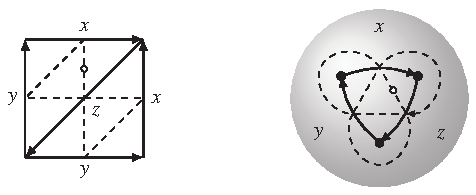
\includegraphics[width=.56\textwidth]{figures/Fig_245_PDF364_Book352.pdf}
  \caption{裤子曲面上的锯齿拉格朗日（原书 p.352）}
  \label{fig:zigzag-lagrangian}
\end{figure}

我们称这个对象为锯齿拉格朗日。作为扭曲复形，它具有如下形式：
\[
  Z=(x\oplus y\oplus z\oplus x\oplus y\oplus z,
  \zeta_1+\xi_2-\eta_1+\zeta_2+\xi_1+\eta_2).
\]
利用引理~\ref{lem:band-self-homs}、引理~\ref{lem:band-intersection-morphisms}、引理~\ref{lem:band-intersection-products} 与引理~\ref{lem:band-higher-product-polygon}，可验证
\[
  E_Z^{\pm}:=\mathrm{topFuk}^{\pm}(Z,Z)
\]
是八维向量空间，由态射 $\iota,\iota^*,p_x,p_y,p_z,p_x^*,p_y^*,p_z^*$ 张成；后六个生成元对应于位于弧 $x,y,z$ 上的三个自交点。若把 $\iota$ 识别为 $1$，把 $p_x,p_y,p_z$ 识别为 $\xi,\eta,\zeta\in\Lambda_3$，则乘积
\[
  \mu(p_x,p_y)=-\mu(p_y,p_x)=p_z^*
\]
可用来把 $p_x^*,p_y^*,p_z^*$ 分别识别为 $\eta\zeta,\zeta\xi,\xi\eta\in\Lambda_3$。最后，乘积 $\mu(p_x,p_x^*)=\iota^*$ 告诉我们 $\iota^*=\xi\eta\zeta$。因此作为代数，$\Lambda_Z$ 同构于外代数 $\Lambda_3$。此外，由引理~\ref{lem:minimal-model-polygon-product} 可知 $\mathrm{topFuk}^{\pm}(Z,Z)$ 带有非平凡的 $A_\infty$ 结构。由于 $\circ$ 与 $\times$ 位于 $x$ 与 $z$ 之间的线段上，有
\[
  \mu(p_x,p_y,p_z)=-\iota.
\]
% [Tutor Note: 此处 $\Lambda_3$ 的下标 $3$ 指生成元 $\xi,\eta,\zeta$ 的个数，而不是分次次数；$p_x^*,p_y^*,p_z^*$ 对应的是 $2$ 次元素 $\eta\zeta,\zeta\xi,\xi\eta$，而 $\iota^*=\xi\eta\zeta$ 对应 $3$ 次元素，它们都住在同一个外代数 $\Lambda_3$ 里，不要误写成 3 次外幂 $\Lambda^3$。]

利用锥构造与 $x,y,z$ 分别对应 $M_X,M_Y,M_Z$ 这一事实，可以在 $\mathrm{MF}^{\pm}(\mathbb C^3,-XYZ)$ 中构造与 $Z$ 对应的对象，并将它与 $(\Omega,\delta+\gamma\wedge)$ 比较；相关矩阵表示见图~\ref{fig:zigzag-matrix-factorization}。直接验证这两个对象拟同构是一个很好的练习，由此可得
\[
  E_Z\cong_\infty E_\gamma\cong_\infty\Lambda_\gamma.
\]
\begin{figure}[H]\centering
  \centering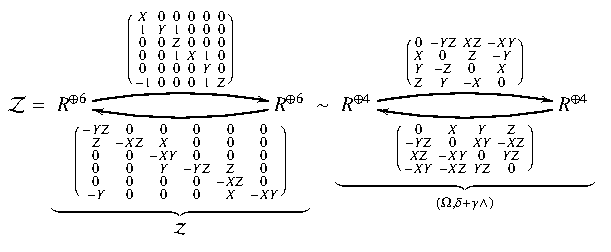
\includegraphics[width=.78\textwidth]{figures/Fig_246_PDF365_Book353.pdf}
  \caption{锯齿对象的矩阵分解表示（原书 p.353）}
  \label{fig:zigzag-matrix-factorization}
\end{figure}

现在填入标记点，考察 $E_Z$ 会发生什么变化。取 $a,b,c>1$ 且为整数，并在三个标记点处分别放置阶数为 $a,b,c$ 的轨形点。记所得曲面为 $S_{abc}$。它的轨形 Euler 示性数为
\[
  \chi=\frac1a+\frac1b+\frac1c-3+2.
\]
有三种可能：
\begin{itemize}
  \item 若 $\chi>0$，则 $S_{abc}$ 可视为球面模某个有限等距群所得的商；
  \item 若 $\chi=0$，则 $S_{abc}$ 可视为欧氏平面模某个晶面等距群所得的商；
  \item 若 $\chi<0$，则 $S_{abc}$ 可视为双曲平面模某个 Fuchsian 群所得的商。
\end{itemize}
在每种情形下，都可以为该曲面定义相对 Fukaya 范畴。$\mathrm{relFuk}^{\pm}(S_{abc})$ 的对象是 $\mathrm{topFuk}^{\pm}(S,\{0,1,\infty\})$ 中的带对象；其乘积计数满足如下条件的全纯映射 $\psi:D\to S_{abc}$：这些映射须经过商构造因子分解。每个映射的权重由局部系统的绕行变换与因子 $\hbar^n$ 决定，其中 $n$ 是圆盘 $D$ 中被映到标记点的点的个数。

在相对 Fukaya 范畴中，锯齿拉格朗日的自同态代数 $E_Z^{\pm}$ 变形为一个可能带曲率的 $A_\infty$ 代数 $E^\hbar_Z$。其中一些变形乘积可以从图~\ref{fig:orbifold-products} 读出。注意，在球面上，$p_x$ 处有两个单边形相接，二者都含有阶数为 $a$ 的轨形点。这些单边形在万有覆盖中提升为 $a$ 边形。其中一个 $a$ 边形上有 $a$ 个 $\circ$，故会产生符号 $(-1)^a$。因此，仿照引理~\ref{lem:band-higher-product-polygon} 与引理~\ref{lem:minimal-model-polygon-product}，有
\[
  \mu_a(p_x,\ldots,p_x)=(-1)^a\hbar\,\iota+\cdots,
  \qquad
  \mu_{a-1}(p_x,\ldots,p_x)=\bigl(\hbar+(-1)^a\hbar\bigr)p_x^*+\cdots,
\]
对 $p_y,p_z$ 也有类似乘积。
\begin{figure}[H]\centering
  \centering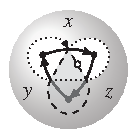
\includegraphics[width=.62\textwidth]{figures/Fig_247_PDF366_Book354.pdf}
  \caption{轨形点在万有覆盖中的多边形提升（原书 p.354）}
  \label{fig:orbifold-products}
\end{figure}

这里仍可区分三种情形：
\begin{itemize}
  \item 若 $\chi>0$，则 $a,b,c$ 中有一个等于 $2$，所以微分可能变为非零。此外，由于万有覆盖是球面，还会出现非平凡的 $\mu_0$。
  \item 若 $\chi=0$，则会有一个阶数为 $2$ 或 $3$ 的轨形点，因此微分会变为非平凡，或者普通乘积会发生变形。另外，若 $a=3$，则 $\mu_{a-1}(p_x,\ldots,p_x)$ 会从尺寸越来越大的三角形得到无穷多个额外贡献。
  \item 若 $\chi<0$，负曲率意味着不存在角度约束相同而尺寸任意大的多边形。因此所有乘积关于 $\hbar$ 都是多项式而非幂级数，我们可以令 $\hbar=1$ 并在 $\mathbb C$ 上工作。若 $a,b,c>3$，所有额外乘积都是高阶乘积；令 $\hbar=1$ 后，$E^\hbar_Z$ 就成为 $E_Z^{\pm}=\Lambda_3$ 的一个 $A_\infty$ 扩张。
\end{itemize}
最后一种情形显然最简单，下面考察它的一个具体例子：令 $a=b=c=2g+1$，其中 $g\geq2$。

\begin{theorem}{Seidel（$g=2$）；Efimov（$g>2$）}{pants-fukaya-landau-ginzburg}
当 $a=b=c=2g+1$ 时，$S_{abc}$ 的 Fukaya 范畴与下列 Landau--Ginzburg 模型分裂导出等价：
\[
  D^{\pi}\mathrm{Fuk}^{\bullet}(S_{abc})
  \cong_\infty D^{\pi}\mathrm{MF}^{\pm}\bigl(\mathbb C^3,
  -XYZ+X^{2g+1}+Y^{2g+1}+Z^{2g+1}\bigr).
\]
\end{theorem}
\begin{proof}[证明思路]
令
\[
  \gamma=-YZ\,dX+X^{2g}\,dX+Y^{2g}\,dY+Z^{2g}\,dZ,
\]
使得
\[
  \delta\gamma=f=-XYZ+X^{2g+1}+Y^{2g+1}+Z^{2g+1}.
\]
把 $p_x,p_y,p_z$ 识别为 $\xi,\eta,\zeta$，并令 $\hbar=1$，则 $E^\hbar_Z$ 与 $\Lambda_\gamma$ 的非零乘积相同：
\[
  \mu_{2g+1}(\xi,\ldots,\xi)
  =\mu_{2g+1}(\eta,\ldots,\eta)
  =\mu_{2g+1}(\zeta,\ldots,\zeta)
  =\iota=-\mu(\xi,\eta,\zeta).
\]
此外，对 $3<k<2g+1$，没有其他非零的 $\mu_k$；这两个 $A_\infty$ 结构都在 $G=\mathbb Z_{2g+1}$ 作用下保持不变，其中 $G$ 对 $\xi,\eta,\zeta$ 的权分别为 $1,1,-2$。

这些性质足以证明 $\Lambda$ 的两个 $A_\infty$ 扩张同构。思路是考察它们在 Hochschild 上同调中的类，并证明二者属于同一轨道。$\Lambda_\gamma$ 的上同调类为
\[
  f=f\otimes1\in\widehat R\otimes\Lambda^{\mathrm{even}}=\mathrm{HH}^1(\Lambda).
\]
由上述乘积可知，$E^\hbar_Z$ 的类形如 $f\otimes1+\cdots$，其中额外项满足 $G$ 不变性，并且只出现在某些次数中。利用 $\widehat R\otimes\Lambda^{\mathrm{odd}}=\mathrm{HH}^0(\Lambda)$ 中适当的元素作用，可以消去这些额外项。更多细节见\bookcite{71}。

为了得到镜像对应，还需证明具有这两个自同态代数的对象都是分裂生成元。对 $(\Omega,\delta+\gamma\wedge)$，这由 Dyckerhoff 的生成判据\bookcite{69} 和 $f$ 只在原点有孤立奇点这一事实推出。对 $Z$，则可使用 Seidel 的生成判据\bookcite{220}。直观上，这是清楚的：$Z$ 把曲面切分为多边形，因此每条曲线都可以同位变形为 $Z$ 上若干线段组成的序列。
\hfill$\square$
\end{proof}

这个镜像对应可以从轨形提升到亏格为 $g$ 的曲面。回忆例~\ref{ex:threefold-pants-cover} 与例~\ref{ex:five-zigzag-dimer}：亏格为 $g$、带三个标记点的曲面 $(S_g,M)$ 到裤子曲面之间存在分歧覆盖，如图~\ref{fig:branched-cover-pants} 所示。该覆盖的自同构群为 $G=\mathbb Z_{2g+1}$，并给出镜像对应
\[
  D^{\pi}\mathrm{topFuk}^{\pm}(\widetilde S,M)
  \cong_\infty D^{\pi}\mathrm{MF}^{\pm}\bigl(\mathbb C[X,Y,Z]\star G,-XYZ\bigr).
\]
\begin{figure}[H]\centering
  \centering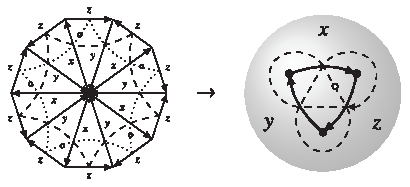
\includegraphics[width=.48\textwidth]{figures/Fig_248_PDF367_Book355.pdf}
  \caption{亏格曲面到裤子曲面的分歧覆盖（原书 p.355）}
  \label{fig:branched-cover-pants}
\end{figure}
锯齿拉格朗日 $Z$ 提升为 $S_g$ 上的 $2g+1$ 条曲线；这些曲线的集合 $\widetilde Z$ 的自同态环为 $E_Z^{\pm}\star G$，它变形为 $E^\hbar_Z\star G$。在 B 侧，函数
\[
  f=-XYZ+X^{2g+1}+Y^{2g+1}+Z^{2g+1}
\]
在 $G$ 作用下不变，故可用它来变形 Landau--Ginzburg 模型 $(\mathbb C[X,Y,Z]\star G,-XYZ)$。与 $S\star G$ 对应的矩阵分解的自同态环为 $\Lambda_\gamma\star G$。由此再次得到两个分裂生成元之间的对应。

\begin{theorem}{Seidel--Efimov}{closed-surface-mirror}
对闭的亏格 $g\geq2$ 曲面，其 Fukaya 范畴与下列两个模型分别分裂导出等价：
\begin{itemize}
  \item 一个带栈 Landau--Ginzburg 模型：
  \[
    D^{\pi}\mathrm{Fuk}^{\pm}(S_g)
    \cong_\infty D^{\pi}\mathrm{MF}^{\pm}\bigl([\mathbb C^3/G],
       -XYZ+X^{2g+1}+Y^{2g+1}+Z^{2g+1}\bigr),
  \]
  其中 $G=\mathbb Z_{2g+1}$ 以权 $(1,1,2g-1)$ 作用在 $\mathbb C^3$ 上；
  \item 一个拟射影 Landau--Ginzburg 模型：
  \[
    D^{\pi}\mathrm{Fuk}^{\pm}(S_g)
    \cong_\infty D^{\pi}\mathrm{MF}^{\pm}\bigl(\widetilde X,
       -XYZ+X^{2g+1}+Y^{2g+1}+Z^{2g+1}\bigr),
  \]
  其中 $\widetilde X$ 是由图~\ref{fig:genus-toric-diagram} 中的扇形图给出的 $\mathbb C^3/\!\!/G$ 的 crepant 解消。
\end{itemize}
\end{theorem}
\begin{figure}[H]\centering
  \centering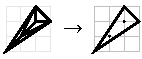
\includegraphics[width=.18\textwidth]{figures/crop_toric_diagram_original_pdf368.pdf}
  \caption{亏格曲面镜像模型的扇形图（原书 p.356）}
  \label{fig:genus-toric-diagram}
\end{figure}
\begin{proof}[证明思路]
带栈版本的证明沿着如下等价链进行：
\[
\begin{aligned}
  D^{\pi}\mathrm{Fuk}^{\pm}(S_g)
  &\cong_\infty D^{\pi}(\Lambda_\gamma\star G)
   \cong_\infty D^{\pi}(E^\hbar_\gamma\star G)\\
  &\cong_\infty D^{\pi}\mathrm{MF}^{\pm}\bigl(\mathbb C[X,Y,Z]\star G,
      -XYZ+X^{2g+1}+Y^{2g+1}+Z^{2g+1}\bigr)\\
  &\cong_\infty D^{\pi}\mathrm{MF}^{\pm}\bigl([\mathbb C^3/G],
      -XYZ+X^{2g+1}+Y^{2g+1}+Z^{2g+1}\bigr).
\end{aligned}
\]
为了得到拟射影版本，可利用 $D^b\mathrm{Coh}\,\widetilde X$ 与 $D^b\mathrm{Coh}[\mathbb C^3/G]$ 之间的导出等价，进而得到两个矩阵分解范畴之间的等价。更多细节见\bookcite{71}。
\hfill$\square$
\end{proof}

\begin{note}[非交换 Landau--Ginzburg 模型]
由引理~\ref{lem:cover-dimer-jacobi-algebra}，还可以使用非交换 Landau--Ginzburg 模型 $(\operatorname{Jac}Q,f)$，其中 $Q$ 是例~\ref{ex:five-zigzag-dimer} 中的二聚体模型，而 $f$ 是同一个函数，不过现在把它看作 $\mathbb C[X,Y,Z]\star G\cong\operatorname{Jac}Q$ 中的中心元。
\end{note}

\begin{example}[亏格为 $1$ 的情形]\label{ex:pants-filling-genus-one}
若亏格为 $1$，同样的技巧给出一个三重覆盖：带三个标记点的环面覆盖带三个标记点的球面。这意味着，产生乘积的 $2g+1$ 边形现在是三角形，因此它们也会贡献到二元乘积中。此外，还存在任意大尺寸的三角形，因此这些贡献成为无穷和。

为了计算乘积，在每个标记点处放置参数 $\hbar$。乘积对给定角点序列的三角形计数：每个三角形中的 $\hbar$ 点贡献因子 $\hbar$；边界上的每个 $\circ$ 贡献局部系统的绕行因子 $\sigma=-1$。于是得到如下二元乘积：
\[
\begin{aligned}
  \mu(\xi,\eta)&=(1+\sigma^3\hbar^3+\sigma^3\hbar^6+\cdots)\zeta^*,\\
  \mu(\eta,\xi)&=(\sigma+\sigma^2\hbar^3+\sigma^4\hbar^6+\cdots)\zeta^*,\\
  \mu(\zeta,\zeta)&=\bigl((1+\sigma^3)\hbar+(\sigma^3+\sigma^6)\hbar^{10}+\cdots\bigr)\zeta^*,
\end{aligned}
\]
并有循环置换得到的类似公式。注意当 $\sigma=-1$ 时，$\mu(\xi,\eta)=-\mu(\eta,\xi)$，且 $\mu(\zeta,\zeta)=0$。不存在形如 $\mu(\xi^*,\eta^*)$ 的乘积，因为它们对应的三角形会有两个钝角。因此，对带星变量作适当缩放后，作为代数，$E^\hbar_Z$ 仍同构于外代数（不过系数环为 $\mathbb C[[\hbar]]$）。图~\ref{fig:torus-triangle-products} 描绘了相关三角形及其乘积。
% [Tutor Note: 这里 $\hbar$ 的幂次 $1,3,6,10$ 正是三角数，对应三角形面积随边长增长；出现 $\hbar^{10}$ 这样的跳跃并非排版错误。]
\begin{figure}[H]\centering
  \centering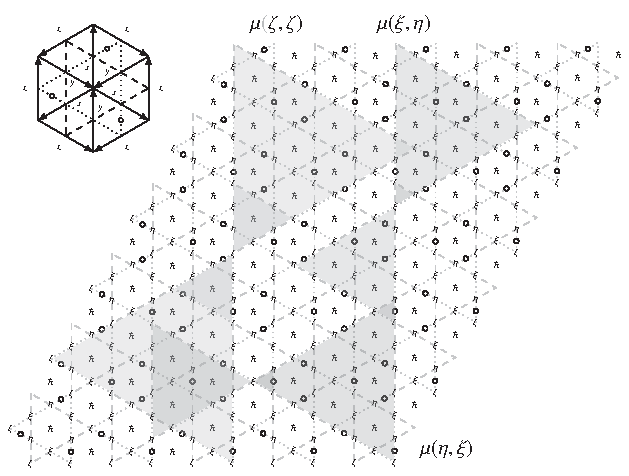
\includegraphics[width=.88\textwidth]{figures/Fig_250_PDF369_Book357.pdf}
  \caption{环面覆盖上的二元乘积（原书 p.357）}
  \label{fig:torus-triangle-products}
\end{figure}

现在考察三元乘积。它们来自经过标记为 $\circ$ 的点的三角形：
\[
\begin{aligned}
  \mu(\zeta,\zeta,\zeta)&=(\sigma^3\hbar+(\sigma^3+2\sigma^6)\hbar^{10}+\cdots)\iota,\\
  \mu(\eta,\xi,\zeta)&=(\sigma+2\sigma^4\hbar^6+\cdots)\iota,\\
  \mu(\xi,\eta,\zeta)&=(\sigma^3\hbar^3+\sigma^6\hbar^6+\cdots)\iota,\\
  &\hspace{2em}\vdots\\
  \mu(\zeta,\eta,\xi)&=(\sigma^3\hbar^3+\sigma^3\hbar^6+\cdots)\iota.
\end{aligned}
\]
因此，若 $E^\hbar_Z$ 同构于 $\Lambda_f$，则 $f$ 具有如下形式：
\[
  (\sigma+\cdots)ZYX+\cdots+(\sigma^3\hbar^3+\cdots)XYZ
  +(\sigma^3\hbar+(\sigma^3+2\sigma^6)\hbar^{10}+\cdots)(X^3+Y^3+Z^3).
\]
把 $XYZ$ 的所有排列项合并，并缩放使其系数为 $1$，便可将 $f$ 化为
\[
  f_\hbar=XYZ+\lambda_\hbar(X^3+Y^3+Z^3),\qquad \lambda_\hbar\in(\hbar).
\]
若选取 $\gamma_\hbar$ 使 $\delta\gamma_\hbar=f_\hbar$，则得到如下两个变形之间的等价：
\[
  E_Z^{\pm}\rightsquigarrow E^\hbar_Z
  \quad\sim\quad
  \Lambda_{\gamma_0}\rightsquigarrow\Lambda_{\gamma_\hbar}.
\]
取扭曲完备化后，得到 $\mathrm{relFuk}^{\pm}(S_{333})$ 与 $\mathrm{MF}^{\pm}(\mathbb C^3,f_\hbar)$ 之间的镜像对应，再与群 $G=\mathbb Z_3$ 作半直积，即可得到带三个已填充标记点的环面之间的镜像对应。这是一个 $\mathbb Z_2$ 分次对应；但环面是 Calabi--Yau 的，因此 Fukaya 范畴可以取 $\mathbb Z$ 分次。

在 B 侧，$f_\hbar$ 是三次齐次函数，故可构造分次矩阵分解范畴。该范畴中存在平移 $S(i)$，分别对应于 $(\Omega(i),\delta+\gamma_\hbar\wedge)$，并且有恒等式 $S(3)=S[2]$；左边的平移来自 $\mathbb C[X,Y,Z]$ 的分次，右边的平移是同调平移。因此矩阵分解范畴 $\mathrm{grMF}^{\bullet}(\mathbb C^3,f_\hbar)$ 由 $S,S(1),S(2)$ 生成。这些对象直和的自同态环作为代数是 $\Lambda\star G$，可写成带关系的箭图路径代数，见图~\ref{fig:graded-matrix-quiver}。
\begin{figure}[H]\centering
  \centering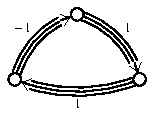
\includegraphics[width=.34\textwidth]{figures/Fig_251_PDF370_Book358.pdf}
  \caption{分次矩阵分解的自同态箭图（原书 p.358）}
  \label{fig:graded-matrix-quiver}
\end{figure}
从各顶点出发的三条箭头表示 $\xi,\eta,\zeta$ 的不同副本。它们的分次取决于起点：前两个副本的次数仍为 $1$，而最后一个副本终止于 $S(3)=S[-2]$，故其次数为 $1-2=-1$。在 Fukaya 一侧，锯齿拉格朗日提升为环面上的三条曲线 $Z_1,Z_2,Z_3$，可适当选择它们的分次，使之与上述次数相配。由此得到 $\mathbb C[[\hbar]]$ 上的 $A_\infty$ 同构
\[
  \operatorname{End}^{\bullet}_{\mathrm{Fuk}}(Z_1\oplus Z_2\oplus Z_3)_\hbar
  \cong_\infty (\Lambda\star G)_\hbar.
\]
取扭曲完备化，并在域 $\mathbb C((\hbar))$ 上工作，便得到
\[
  D^{\pi}\mathrm{Fuk}^{\bullet}(T,M)_{\mathbb C((\hbar))}
  \cong_\infty D^{\pi}\mathrm{grMF}\bigl(\mathbb C((\hbar))[X,Y,Z],f_\hbar\bigr).
\]

由 Orlov 定理（定理~\ref{thm:orlov-hypersurface}），右侧与
\[
  \mathrm{P}\bigl(\mathbb C((\hbar))[X,Y,Z]/(f_\hbar)\bigr)
\]
导出等价；后者是椭圆曲线族的一般成员。当 $\hbar\to0$ 时，该族退化为
\[
  \mathrm{P}\bigl(\mathbb C[X,Y,Z]/(XYZ)\bigr),
\]
这是一条带三个节点奇点、由三条 $\mathbb P^1$ 串接而成的曲线。该退化可看成曲面上的三条曲线收缩到一点；这些消失圈对应 A 侧的标记点。图~\ref{fig:elliptic-degeneration} 示意了 A 侧与 B 侧的退化。
\begin{figure}[H]\centering
  \centering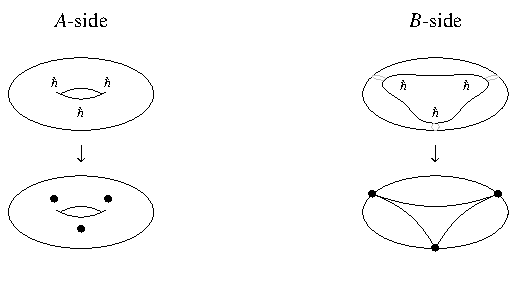
\includegraphics[width=.7\textwidth]{figures/Fig_252_PDF371_Book359.pdf}
  \caption{椭圆曲线镜像族的退化（原书 p.359）}
  \label{fig:elliptic-degeneration}
\end{figure}
\end{example}

\begin{note}[椭圆曲线的镜像对称]
许多数学家研究过椭圆曲线的镜像对称，下面列出几个例子。
\begin{itemize}
  \item 环面的原始镜像对应（以 $\mathbb C$ 上的导出范畴表述，而不着重考察 $A_\infty$ 结构）由 Polishchuk 与 Zaslow 给出\bookcite{205}。
  \item 上述构造由 Cho、Hong 与 Lau 在\bookcite{55} 中详细研究；他们使用 Novikov 环上的完整 Fukaya 范畴，从而得到以面积参数表示的不同 $\lambda_\hbar$。
  \item 环面的相对观点方面，Lekili 与 Perutz 研究了一个标记点的情形\bookcite{162,161}；Lekili 与 Polishchuk 研究了多个标记点的情形\bookcite{164}。后一种工作使用另一组拉格朗日 brane，将环面切成若干矩形，每个矩形包含一个标记点，并各自带有变形参数 $t_i$。图~\ref{fig:torus-relative-mirror} 展示了 A 侧与 B 侧的构造。
\end{itemize}
\begin{figure}[H]\centering
  \centering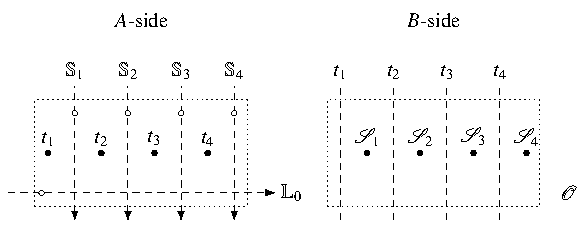
\includegraphics[width=.77\textwidth]{figures/Fig_253_PDF371_Book359.pdf}
  \caption{带多个标记点的环面上的相对镜像构造（原书 p.359）}
  \label{fig:torus-relative-mirror}
\end{figure}
当 $n=1$ 时，镜像族可视为由方程
\[
  Y^2Z+XYZ=X^3+a(\hbar)XZ^2+b(\hbar)Z^3
\]
定义的 Weierstrass 族。当 $\hbar\to0$ 时，它退化为结点曲线 $Y^2Z+XYZ=X^3$。对带 $n$ 个标记点的环面，相应族是 Tate 曲线；它退化为由 $n$ 条射影直线组成的链。

与拉格朗日 $L_0$ 镜像对应的对象是曲线的结构层；与 $S_i$ 镜像对应的对象则是点的 skyscraper 层。它们的自同态环是如下带关系路径代数的一个 $A_\infty$ 扩张：图~\ref{fig:torus-relative-quiver}。
\begin{figure}[H]\centering
  \centering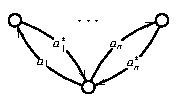
\includegraphics[width=.45\textwidth]{figures/Fig_254_PDF372_Book360.pdf}
  \caption{相对镜像对象的箭图关系（原书 p.360）}
  \label{fig:torus-relative-quiver}
\end{figure}
其关系为 $a_i^*a_i=a_j^*a_j$ 且 $a_i a_j^*=0$。与锯齿拉格朗日的情形类似，即使令 $\hbar=0$，这个 $A_\infty$ 扩张仍然非平凡。

值得注意的是，此构造具有一种特殊对称性：A 侧的每个标记点都对应 B 侧的一条消失圈，而 B 侧每个带标记的 skyscraper 层都对应 A 侧的一条拉格朗日圈。
\end{note}

本节最后介绍一个非交换镜像构造。在计算 $S_{333}$ 的乘积时，我们特意把符号写成 $\sigma$，因为现在要稍作不同处理：不再给 $Z$ 赋予非平凡自旋结构，而是给它配备绕行变换为 $\rho\ne-1$ 的局部系统。记新的拉格朗日 brane 为 $Z_\rho$，它在环面上的提升为 $\widetilde Z_\rho$，其自同态环记作 $E^\hbar_{Z_\rho}$。

为了确定这个自同态环，可以沿用上述计算，只需把 $\sigma$ 换成 $\rho$。所得外代数 $\Lambda$ 上出现了新的代数结构：现在 $\mu(\zeta,\zeta)$ 不再为零，而且 $\mu(\xi,\eta)$ 的系数也不同。确切地说，存在 $\alpha,\beta,\gamma\in\mathbb C[[\hbar]]$，使二元乘积为
\[
\begin{array}{c|ccc}
  \cdot & \xi & \eta & \zeta\\\hline
  \xi & \gamma\xi^* & \beta\zeta^* & \alpha\eta^*\\
  \eta & \alpha\zeta^* & \gamma\eta^* & \beta\xi^*\\
  \zeta & \beta\eta^* & \alpha\xi^* & \gamma\zeta^*
\end{array}
\]
把这个不带高阶乘积的新代数记作 $\Lambda_{\alpha\beta\gamma}$，于是 $E^\hbar_{Z_\rho}$ 是 $\Lambda_{\alpha\beta\gamma}$ 的一个 $A_\infty$ 扩张。$\Lambda_{\alpha\beta\gamma}$ 中的乘积提示，它是另一个代数的 Koszul 对偶：
\[
\begin{aligned}
  \Lambda_{\alpha\beta\gamma}&=\operatorname{Ext}_A(S,S),\\
  A=Skl_{\alpha\beta\gamma}&:=
  \frac{\mathbb C\langle X,Y,Z\rangle}
  {\left\langle\begin{gathered}
    \alpha XY+\beta YX+\gamma Z^2,\\
    \alpha YZ+\beta ZY+\gamma X^2,\\
    \alpha ZX+\beta XZ+\gamma Y^2
  \end{gathered}\right\rangle}.
\end{aligned}
\]
遗憾的是，这并非总是成立，因为该代数可能没有有限整体维数；但对一般的 $\alpha,\beta,\gamma$，结论成立。这些代数称为三维 Sklyanin 代数\index{sklyanindaishu@Sklyanin 代数|hyperpage}，可视为三变量多项式环的良好非交换变形。

Artin、Tate 与 Van den Bergh 研究了这些代数\bookcite{17}，并证明这类环的中心由一个次数为 $3$ 的元素 $\ell$ 生成。商 $Skl_{\alpha\beta\gamma}/\langle\ell\rangle$ 有良好的几何描述：它是椭圆曲线的扭曲坐标环。更精确地说，存在椭圆曲线 $E$、线丛 $L$ 及自同构 $\tau:E\to E$，使得
\[
  B=\frac{\operatorname{Skl}_{\alpha\beta\gamma}}{\langle\ell\rangle}
  \cong\bigoplus_{r=0}^{\infty}
  L\otimes L^\tau\otimes\cdots\otimes L^{\tau^{r-1}}(E),
\]
且乘法为 $u\cdot v=u\otimes\tau^{\deg u}(v)$（$\tau$ 通过拉回作用在线丛上）。从非交换代数几何角度，可把 $A$ 看作非交换射影平面 $\mathbb P_{\alpha\beta\gamma}$ 的齐次坐标环，而椭圆曲线嵌在该射影平面中。对这两个对象可定义凝聚层范畴：
\[
  \operatorname{Coh}\mathbb P_{\alpha\beta\gamma}
  :=\frac{\operatorname{grMod}A}{\operatorname{grmod}A},\qquad
  \operatorname{Coh}E_{\alpha\beta\gamma}
  :=\frac{\operatorname{grMod}B}{\operatorname{grmod}B}.
\]
需要强调，虽然 $\operatorname{Coh}\mathbb P_{\alpha\beta\gamma}$ 不等价于某个交换簇的凝聚层范畴，但 $\operatorname{Coh}E_{\alpha\beta\gamma}$ 与上述椭圆曲线 $E$ 的凝聚层范畴等价。

令人惊讶的是，这个元素 $\ell$ 正是利用三元乘积求得的 $f_\hbar$。若在奇点范畴
\[
  \operatorname{Sing}^{\bullet}B\cong_\infty D^{\pi}\mathrm{MF}^{\bullet}(A,f_\hbar)
\]
中计算简单 $B$ 模 $S=B/\langle X,Y,Z\rangle$ 的自同态环，可得 $E^\hbar_S$；它是 $\Lambda_{\alpha\beta\gamma}$ 的一个 $A_\infty$ 扩张，并与 $E^\hbar_{Z_\rho}$ 等价。结合 Orlov 定理的非交换版本（定理~\ref{thm:orlov-hypersurface}），得到如下等价链：
\[
\begin{aligned}
  D^{\pi}\mathrm{Fuk}^{\bullet}(T,M)_{\mathbb C((\hbar))}
  &\cong_\infty D^{\pi}E^\hbar_{\widetilde Z_\rho}
   \cong_\infty D^{\pi}(E^\hbar_{Z_\rho}\star\mathbb Z_3)
   \cong_\infty D^{\pi}(E^\hbar_S\star\mathbb Z_3)\\
  &\cong_\infty D^{\pi}\mathrm{grMF}^{\bullet}(A,f_\hbar)
   \cong_\infty\frac{D^b\mathrm{grMod}^{\bullet}B}{D^b\mathrm{Perf}^{\bullet}B}
   \cong_\infty\frac{D^b\mathrm{grMod}^{\bullet}B}{D^b\mathrm{grmod}^{\bullet}B}
   \cong_\infty D^{\infty}\mathrm{Coh}^{\bullet}E.
\end{aligned}
\]


这一结果可以这样理解：无论交换情形还是非交换情形，环面的镜像都可以看作嵌在射影平面中的椭圆曲线，是某个齐次函数的零点：
\[
  E=\mathrm P\bigl(\mathbb C((\hbar))[X,Y,Z]/(f_\hbar)\bigr)
  \subset\mathbb P^2=\mathrm P\bigl(\mathbb C((\hbar))[X,Y,Z]\bigr),
\]
\[
  E=\mathrm P\bigl(Skl^{\hbar}_{\alpha\beta\gamma}/\langle f_\hbar\rangle\bigr)
  \subset\mathbb P^2_{\alpha\beta\gamma}
  =\mathrm P\bigl(Skl^{\hbar}_{\alpha\beta\gamma}\bigr).
\]
Cho、Hong 与 Lau 在\bookcite{154} 中用更一般的框架发展了这些思想；接下来两节将讨论该框架。

\section{Koszul 对偶}\label{sec:koszul-duality}

我们先简要讨论 Koszul 对偶\index{koszulduiou@Koszul 对偶|hyperpage}。有关这一主题的更多信息，参见 Beilinson、Ginzburg 与 Soergel 的工作\bookcite{27}；关于它与 $A_\infty$ 代数的联系，可参见\bookcite{167,249}。
\takeaway{Koszul 对偶把以顶点为严格单位元的 $A_\infty$ 结构 $(\Lambda_Q,\mu)$ 一一对应到完备路径代数 $\widehat{\mathbb C Q}$ 上的微分分次结构 $\mu\mapsto d_\mu$，其中 $A_\infty$ 公理恰等价于 $d_\mu^2=0$；它还给出有限维右 $A_\infty$ 模范畴与 $A^!$ 的扭曲复形范畴的等价。}

设 $Q$ 是一个箭图，记其完备路径代数为 $\widehat{\mathbb C Q}$，其对偶箭图代数为 $\Lambda_Q$。回忆
\[
  \Lambda_Q=\operatorname{Ext}^{\bullet}_{\mathbb C Q}(S,S)
  =\mathbb C Q^{\mathrm{op}}/\langle\alpha\beta\mid\alpha,\beta\in Q_1^{\mathrm{op}}\rangle,
\]
其中 $S=\widehat{\mathbb C Q}/\langle a\in Q_1\rangle$。换言之，$Q$ 中每个箭头 $a$ 都对应于 $\Lambda_Q$ 中方向相反的对偶箭头 $\alpha$，并且所有乘积 $\alpha\beta$ 都为零。因此，作为向量空间，$\Lambda_Q$ 由顶点和对偶箭头张成。

$Q$ 中箭头与 $Q^{\mathrm{op}}$ 中箭头之间的配对延拓为路径之间的配对：若 $p=a_1\cdots a_k$ 是 $Q$ 中的一条路径，则记
\[
  p^\vee=\alpha_k\otimes\cdots\otimes\alpha_1
  \in(\mathbb C Q^{\mathrm{op}})_k=(\Lambda_Q)^{\otimes k},
\]
其中张量积分别在 $\mathbb C Q_0$ 与 $\mathbb C Q_0^{\mathrm{op}}$ 上取。

在 $\Lambda_Q$ 的箭头上选取一个正的 $\mathbb Z$ 分次 $\deg:Q_1^{\mathrm{op}}\to\mathbb N$，并在 $\Lambda_Q$ 上取一个 $A_\infty$ 结构 $\mu$，使顶点在把 $(\Lambda_Q,\mu)$ 看成 $A_\infty$ 范畴时成为严格单位元。给完备路径代数 $\widehat{\mathbb C Q}$ 赋予对偶分次
\[
  \deg a=1-\deg\alpha,
\]
并定义微分 $d_\mu:\widehat{\mathbb C Q}\to\widehat{\mathbb C Q}$，使得对每个 $a\in Q_1$，
\[
  d_\mu a=\sum_p\mu(p^\vee)(a)\,p,
\]
求和遍历 $Q$ 中所有路径。也就是说，路径 $a_1\cdots a_k$ 在 $d_\mu a$ 中的系数，等于 $\alpha_k,\ldots,\alpha_1$ 的乘积 $\mu(\alpha_k,\ldots,\alpha_1)$ 中 $\alpha$ 的系数。由于 $\widehat{\mathbb C Q}$ 没有关系，可按分次 Leibniz 规则把 $d_\mu$ 延拓到整个代数。按这一新分次，$d_\mu$ 的次数为 $1$，且 $\widehat{\mathbb C Q}$ 在正次数部分为零。

\begin{theorem}{$A_\infty$ 代数的 Koszul 对偶}{koszul-duality-ainfty-algebras}
赋值 $\mu\mapsto d_\mu$ 给出如下两类对象之间的一一对应：
\begin{itemize}
  \item 顶点为严格单位元的 $A_\infty$ 结构 $(\Lambda_Q,\mu)$；
  \item 完备路径代数 $\widehat{\mathbb C Q}$ 上的微分分次结构。
\end{itemize}
\end{theorem}
\begin{proof}[证明思路]
关键观察是，$\mu$ 的 $A_\infty$ 公理等价于 $d_\mu^2=0$。
\hfill$\square$
\end{proof}

\begin{definition}{Koszul 对偶}{koszul-dual-algebra}
称 $A^!=(\widehat{\mathbb C Q},d_\mu)$ 为 $A=(\Lambda_Q,\mu)$ 的 Koszul 对偶。
\end{definition}

\begin{example}[二变量外代数的 Koszul 对偶]
令 $A=\Lambda_2=\mathbb C\oplus\mathbb C\xi\oplus\mathbb C\eta\oplus\mathbb C\rho$ 为二变量外代数，其中 $\rho=\xi\eta=-\eta\xi$。此时 $Q^{\mathrm{op}}$ 有一个顶点和三个自环 $\xi,\eta,\rho$，且 $\mu(\xi,\eta)=-\mu(\eta,\xi)=\rho$。其 Koszul 对偶为
\[
  \mathbb C\langle\!\langle X,Y,R\rangle\!\rangle,
  \qquad dX=dY=0,\quad dR=XY-YX,
\]
其中 $\deg X=\deg Y=0$、$\deg R=-1$。这个微分分次代数的同调为集中在次数 $0$ 的 $\mathbb C[[X,Y]]$，因此 $A^!$ 与 $\mathbb C[[X,Y]]$ 作为代数拟同构。
\end{example}

Koszul 对偶的 $A_\infty$ 代数之间的乘积密切相关；这也反映在它们的表示论中。

\begin{theorem}{模的 Koszul 对偶}{koszul-duality-modules}
存在如下等价：$A$ 的有限维右 $A_\infty$ 模范畴与 $A^!$ 的扭曲复形范畴等价，反之亦然：
\[
  \mathrm{mod}_{\infty}^{\bullet}A\cong_\infty\mathrm{Tw}A^!,\qquad
  \mathrm{mod}_{\infty}^{\bullet}A^!\cong_\infty\mathrm{Tw}A.
\]
\end{theorem}
\begin{proof}[证明思路]
简要说明 $A$ 只是一个代数（即箭图只有一个顶点）的情形；一般情形相似，但写起来更繁复。$A$ 的每个有限维 $A_\infty$ 模都可看成一个 $A_\infty$ 态射
\[
  F_{\bullet}:A^{\mathrm{op}}\to\operatorname{Mat}_{n\times n}^{\bullet}(\mathbb C)
  =\operatorname{End}_{\mathrm{grvect}^{\bullet}}(V),
\]
其中 $V$ 是有限维分次向量空间。由于 $A$ 正分次，可以假定这些矩阵映射是下三角的。

沿用前面的构造，可定义一个取值于 $A^!$ 的矩阵
\[
  \delta_F=\sum_p F(p^\vee)\otimes p
  \in\operatorname{Mat}_{n\times n}(A^!)
  =\operatorname{End}_{\mathrm{grvect}^{\bullet}}(V)\otimes A^!.
\]
$F$ 满足 $A_\infty$ 关系，等价于 $\delta_F$ 满足 Maurer--Cartan 方程
\[
  d_\mu\delta_F+\delta_F^2=0.
\]
因此，我们得到 $V$ 与扭曲复形 $(A^!\otimes V,\delta_F)$ 之间的对应。

反过来，令 $S$ 为生成元作用为零的简单 $A^!$ 模。可证明
\[
  \operatorname{Ext}^{\bullet}_{A^!}(S,S)\cong_\infty A.
\]
由于 $A^!$ 是完备的，$S$ 生成所有有限维模，因此 $\mathrm{mod}_{\infty}^{\bullet}A^!=\langle S\rangle^{\infty}\cong_\infty\mathrm{Tw}A$。
\hfill$\square$
\end{proof}

$\mathrm{mod}_{\infty}^{\bullet}A$ 与 $\mathrm{Tw}A^!$ 的识别也可用于把其他范畴映到 $A^!$ 的扭曲复形范畴。若 $A^{\bullet}$ 是较大范畴 $\mathcal C^{\bullet}$ 的子范畴，且从 $A$ 出发的所有 Hom 空间都是有限维的，则可把 $\mathcal C^{\bullet}$ 中每个对象 $X$ 看成右 $A_\infty$ 模
\[
  F_X:A^{\bullet}\to\operatorname{End}^{\bullet}_{\mathcal C}
  \bigl(\mathcal C^{\bullet}(A,X)\bigr),\qquad
  F_X(\alpha_1\otimes\cdots\otimes\alpha_n)(\xi)
  :=F_X(\alpha_n,\ldots,\alpha_1,\xi).
\]
将它与前述识别复合，得到一个 $A_\infty$ 函子
\[
  K_A:\mathcal C^{\bullet}\longrightarrow\mathrm{Tw}A^!.
\]

\begin{example}[点模的像]
取简单 $\mathbb C[X,Y]$ 模 $S=\mathbb C[X,Y]/(X,Y)$，并把它的 Ext 代数
\[
  A=\operatorname{Ext}^{\bullet}_{\mathbb C[X,Y]}(S,S)=\Lambda_2
\]
看成 $\mathrm{mod}^{\bullet}\mathbb C[X,Y]$ 的子范畴。这给出函子
\[
  K_A:\mathrm{mod}^{\bullet}\mathbb C[X,Y]\to\mathrm{Tw}\Lambda_2^!.
\]
现在已知 $\Lambda_2^!$ 与完备多项式环 $\mathbb C[[X,Y]]$ 拟同构，因此得到函子
\[
  \mathrm{mod}^{\bullet}\mathbb C[X,Y]\longrightarrow\mathrm{Tw}\mathbb C[[X,Y]].
\]
该函子把 $S$ 映到一个有 $\dim\Lambda_2=4$ 个直和项的扭曲复形，也就是 $S$ 作为 $\mathbb C[[X,Y]]$ 模的标准分解。由于其他任意简单 $\mathbb C[X,Y]$ 模与 $S$ 之间的 Ext 代数为零，这些简单模都被映到零复形。
\end{example}

\begin{example}[无环箭图的 Koszul 对偶函子]
若 $Q$ 是无有向环箭图，且 $S^{\bullet}$ 是简单模构成的子范畴，则 $A^!=\mathbb C Q$。函子 $K_{S^{\bullet}}$ 把 $\mathbb C Q$ 的模 $S_\rho$ 映到它的分解 $P_\rho$，所以 $K_{S^{\bullet}}$ 是等价。若 $Q$ 含有有向环，则 $S_\rho$ 被映到 $S_\rho\otimes_{\mathbb C Q}\widehat{\mathbb C Q}$ 的分解。
\end{example}

\begin{note}[局部化视角]
函子 $K_A:\mathcal C^{\bullet}\to\mathrm{Tw}A^!$ 应理解为某种局部化。若对象 $X$ 满足 $\mathcal C^{\bullet}(A,X)=0$（换言之，$X$ 与 $A$ 并不接近），则 $K_A$ 会把 $X$ 消去。

若 $A^{\pm}$ 是 $\mathbb Z_2$ 分次，则情况会改变，因为这时可能出现含顶点的乘积，例如 $\mu(\alpha,\alpha,\alpha)=v$。对偶地，这意味着 $d_\mu v=a^3$，因此 $v$ 不再是该微分分次代数的严格单位元。此外，构造中的扭曲复形也不再是下三角的，因为 $A^{\pm}$ 并非正分次。为了处理这些问题，我们将构造 $A^!$ 的替代物——Landau--Ginzburg 模型，并使局部函子以矩阵分解而非扭曲复形为值。下面针对本书相关的情形给出细节。
\end{note}

\section{镜像函子}\label{sec:mirror-functor}
\takeaway{镜像函子 $F:\mathcal C^{\pm}\to\mathrm{MF}^{\pm}(A,\ell)$ 把对象 $X$ 送到 $\bigl(A\otimes\mathcal C^{\pm}(B,X),d\bigr)$，其中 $dx=\mu(x)+\mu(x,b)+\cdots$ 满足 $d^2x=\ell x$，即像自动是 Landau--Ginzburg 模型的矩阵分解；它由锯齿骨架与二聚体给出，并在双重一致情形猜想为等价。}

令
\[
  B=(B_1,\rho_1)\oplus\cdots\oplus(B_k,\rho_k)
\]
是拓扑 Fukaya 范畴中的一组带对象。选取标记 $\circ,\ast,\times$，以确定其自同态 $A_\infty$ 代数 $E_B^{\pm}$ 的极小模型。作为向量空间，它由以下基元素张成：
\begin{itemize}
  \item 恒等态射 $\iota_1,\ldots,\iota_k$，分别对应带上的 $\circ$ 标记；
  \item 次数为 $1$ 的态射 $\alpha_1,\ldots,\alpha_\ell$，每个交点对应一个；
  \item 次数为 $0$ 的态射 $\alpha_1^*,\ldots,\alpha_\ell^*$，每个与 $\alpha_i$ 方向相反的交点对应一个；
  \item 次数为 $1$ 的态射 $\iota_1^*,\ldots,\iota_k^*$，分别对应带上的 $\ast$ 标记。
\end{itemize}
把 $\iota_1,\ldots,\iota_k$ 看成某个箭图的顶点，把 $\alpha_1,\ldots,\alpha_\ell$ 看成箭头。令 $v_1,\ldots,v_k$ 与 $a_1,\ldots,a_\ell$ 分别为对偶箭图的顶点和箭头，并记该对偶箭图为 $Q$。注意，与 Koszul 对偶的构造不同，$Q$ 只包含 $E_B^{\pm}$ 中无星部分的对偶。从另一角度看，也可以说我们消去了带星部分：作为代数，
\[
  \mathbb C Q=(E_B^{\pm})^!/I^*,
\]
其中 $I^*\subset(E_B^{\pm})^!$ 是由 $\alpha_i^*$ 与 $\iota_j^*$ 的对偶生成元生成的理想。

在 $\widehat{\mathbb C Q}$ 中定义以下元素：
\begin{itemize}
  \item 对每个顶点 $v\in Q_0$，令
  \[
    \ell_v=\sum_p\mu(p^\vee)(v)p;
  \]
  \item 对每个箭头 $a\in Q_1$，令
  \[
    r_a=\sum_p\mu(p^\vee)(a^*)p.
  \]
\end{itemize}
以上两式的求和都遍历 $Q$ 中的所有路径。这些元素记录了 Koszul 微分中无星部分：
\[
  \ell_v=d_\mu(v)\bmod I^*,\qquad r_i=d_\mu(a_i^*)\bmod I^*.
\]

\begin{theorem}{Cho--Hong--Lau}{cho-hong-lau-landau-ginzburg}
有序对
\[
  (A,\ell):=
  \left(\frac{\widehat{\mathbb C Q}}{\langle r_1,\ldots,r_k\rangle},
  \sum_v\ell_v\right)
\]
是一个非交换 Landau--Ginzburg 模型。
\end{theorem}
\begin{proof}[证明思路]
一个简洁的证明方法，是把 $E_B^{\pm}$ 上的 $A_\infty$ 结构延拓到 $A\otimes_{\Bbbk}E_B^{\pm}$ 上，规定
\[
  \mu(p_1\otimes\gamma_1,\ldots,p_k\otimes\gamma_k)
  =p_k\cdots p_2p_1\otimes\mu(\gamma_1,\ldots,\gamma_k).
\]
容易验证这一定义满足 $A_\infty$ 公理。现在令 $b=\sum_i a_i\otimes\alpha_i$，则
\[
  \sum_{k\geq1}\mu_k(b,\ldots,b)
  =\sum_v\ell_v\otimes\iota_v+\sum_jr_j\otimes\alpha_j^*
  =\sum_v\ell_v\otimes\iota_v,
\]
因为在 $A$ 中 $r_j=0$。结合 $A_\infty$ 公理与 $\iota_i$ 是严格单位元这一事实，有
\begin{align*}
  0&=\sum\pm\mu_k\bigl(b,\ldots,b,\mu_l(b,\ldots,b),b,\ldots,b\bigr)\\
   &=\sum\mu_2\left(b,\sum_v\ell_v\otimes\iota_v\right)
     -\sum\mu_2\left(\sum_v\ell_v\otimes\iota_v,b\right)\\
   &=\sum_j\bigl(\ell_{h(a_j)}a_j-a_j\ell_{t(a_j)}\bigr)\otimes\alpha_j.
\end{align*}
所以 $\sum_v\ell_v$ 与每个 $a_j$ 交换，因而是中心元。更多信息见\bookcite{154}。
\hfill$\square$
\end{proof}

若 $E_B^{\pm}$ 嵌在较大的范畴 $\mathcal C^{\pm}$ 中，可构造 $A_\infty$ 函子
\[
  F:\mathcal C^{\pm}\longrightarrow\mathrm{MF}^{\pm}(A,\ell),\qquad
  X\longmapsto\bigl(A\otimes\mathcal C^{\pm}(B,X),d\bigr),
\]
其中
\[
  dx=\mu(x)+\mu(x,b)+\mu(x,b,b)+\cdots.
\]
由 $A_\infty$ 关系
\[
\begin{aligned}
  0&=\sum\mu\bigl(\mu(x,b,\ldots,b),b,\ldots,b\bigr)
  +\sum\mu\bigl(x,\mu(b,\ldots,b),b,\ldots,b\bigr)+\cdots\\
   &=d^2x+\mu(x,\ell\otimes1)+\mu(x,b,\ldots,\ell\otimes1,\ldots,b)+\cdots\\
   &=d^2x-\ell x.
\end{aligned}
\]
函子的高阶部分为
\[
  F_k(c_1,\ldots,c_k)=\sum\mu(c_1,\ldots,c_k,b,\ldots,b).
\]

\begin{theorem}{Cho--Hong--Lau}{cho-hong-lau-mirror-functor}
若所有 Hom 空间 $\mathcal C^{\pm}(B,X)$ 都是有限维的，则
\[
  F_{\bullet}:\mathcal C^{\pm}\longrightarrow\mathrm{MF}^{\pm}(A,\ell)
\]
是一个 $A_\infty$ 函子。
\end{theorem}
\begin{proof}[证明思路]
证明与定理~\ref{thm:cho-hong-lau-landau-ginzburg} 类似，也可参见\bookcite{154}。
\hfill$\square$
\end{proof}

\begin{example}[裤子曲面上的镜像函子]
回到第~\ref{sec:filling-pants} 节开头描述的裤子曲面锯齿拉格朗日 $Z$。考察 $E_Z^{\pm}$ 可得
\[
  \ell=-XYZ,\qquad r_1=XZ-ZX,\quad r_2=ZY-YZ,\quad r_3=YX-XY.
\]
因此 Landau--Ginzburg 模型为 $(\mathbb C[[X,Y,Z]],-XYZ)$。取弧 $x$，考察它在函子
\[
  F:\mathrm{topFuk}^{\pm}(S,\{0,1,\infty\})
  \longrightarrow\mathrm{MF}^{\pm}(\mathbb C[[X,Y,Z]],-XYZ)
\]
下的像。稍微扰动弧后可见两个交点 $p,q$，它们分别给出次数为 $0$ 和 $1$ 的态射。由图~\ref{fig:mirror-functor-pants-arc} 可读出两个非平凡乘积
\[
  \mu(q,\xi)=p,\qquad \mu(p,\eta,\zeta)=-q,
\]
从而 $dp=Xq$、$dq=-YZp$。因此
\[
  F(x)=\left(\mathbb C[[X,Y,Z]]^{\oplus2},
  \begin{pmatrix}0&X\\-YZ&0\end{pmatrix}\right).
\]
绕某个标记点的带对象与锯齿拉格朗日不相交，所以被映到零对象。
\begin{figure}[H]\centering
  \centering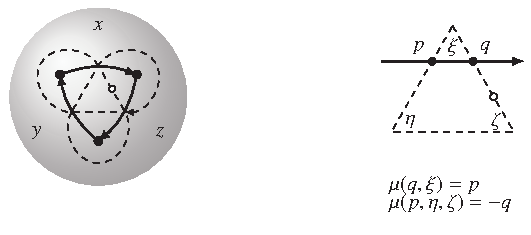
\includegraphics[width=.78\textwidth]{figures/Fig_255_PDF379_Book367.pdf}
  \caption{裤子曲面上的镜像函子与弧的像（原书 p.367）}
  \label{fig:mirror-functor-pants-arc}
\end{figure}
\end{example}

\begin{example}[填充裤子曲面上的镜像函子]
若把裤子曲面的锯齿拉格朗日嵌入带三个轨形点的球面，就得到 Landau--Ginzburg 模型
\[
  (\mathbb C[[X,Y,Z]],-XYZ+X^{2g+1}+Y^{2g+1}+Z^{2g+1}).
\]
镜像函子把锯齿拉格朗日本身映到 $(\mathbb C[[X,Y,Z]]\otimes\Lambda_3,d)$，其中
\[
\begin{aligned}
  d\iota&=X\xi+Y\eta+Z\zeta,\\
  d\xi&=-YZ\iota+Z\eta-Y\zeta,\\
  &\hspace{2em}\vdots\\
  d\zeta^*&=Z\iota^*-Y\xi+X\eta,\\
  d\iota^*&=(X^{2g}-YZ)\xi^*+(Y^{2g}-XZ)\eta^*+(Z^{2g}-XY)\zeta^*.
\end{aligned}
\]
这恰好就是 $(\Omega,\delta+\gamma\wedge)$。由于镜像函子与锥构造相容，并且 $Z$ 与 $(\Omega,\delta+\gamma\wedge)$ 都是生成元，因此在此情形下镜像函子是等价。
\end{example}

\begin{example}[锯齿拉格朗日]
取亏格为 $g$、有 $n$ 个内部标记点的闭带标记曲面 $(S,M)$，并取构成二聚体的弧系 $A$，把它的镜像记作 $Q$，故 $A=Q^{\vee}$。按照\bookcite[第 10 节]{154}，还需取符号映射
\[
  \rho:(Q_A)_1\to\{+1,-1\},
\]
使得每个具有奇数个角的顺时针多边形都恰含一个负号角箭头，其余角箭头的符号均为正。

从一条弧出发，沿锯齿路径继续前进，直到路径重复。把各弧的中点连接起来，便得到一条闭曲线。对每条这样的曲线构造复形
\[
  Z_i=(a_1\oplus\cdots\oplus a_k,
  \rho(\alpha_1)\alpha_1+\cdots+\rho(\alpha_k)\alpha_k)
  \in\mathrm{topFuk}^{\pm}(S,M).
\]
锯齿骨架 $Z$ 是所有 $Z_i$ 的直和。对每个锯齿圈，还要固定一条标记弧 $a_1$ 和一个标记角 $\alpha_1$，以便构造极小模型。按照第~\ref{note:ribbon-graph-skeleton}~节的注，在 $a_1$ 后方的曲线上放置 $\circ,\ast$；每个满足 $\rho(\alpha)=-1$ 的角还放置一个 $\times$。图~\ref{fig:zigzag-skeleton-construction} 展示了这一构造。
\begin{figure}[H]\centering
  \centering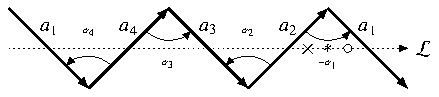
\includegraphics[width=.58\textwidth]{figures/Fig_256_PDF380_Book368.pdf}
  \caption{锯齿曲线与锯齿拉格朗日（原书 p.368）}
  \label{fig:zigzag-skeleton-construction}
\end{figure}
\end{example}

\begin{theorem}{Cho--Hong--Lau}{zigzag-dimer-mirror}
与锯齿骨架 $Z$ 相关的 Landau--Ginzburg 模型由对偶二聚体的完备 Jacobi 代数与其中心元 $\ell$ 构成：
\[
  (\widehat{\operatorname{Jac}}\,Q,\ell).
\]
\end{theorem}
\begin{proof}[证明思路]
每条弧 $a$ 恰属于两个多边形 $a_1\cdots a_k$ 与 $b_1\cdots b_\ell$，其中 $b_1=a_1=a$；它们给出两个非零乘积
\[
  \mu(\alpha_2,\ldots,\alpha_k)
  =-\mu(\beta_2,\ldots,\beta_\ell)=\alpha^*,
\]
由于符号映射 $\rho$ 的选取，这两个乘积符号相反。对偶地，
\[
  r_a=a_k\cdots a_2-b_\ell\cdots b_2,
\]
这恰好是定义~\ref{def:jacobi-algebra} 中对偶二聚体 Jacobi 代数的关系。为了确定 $\ell$，只需注意每个 $\circ$ 恰落在一个多边形中，所以 $\ell$ 是每个顶点各取一个多边形环的和，与引理~\ref{lem:jacobi-central-element} 相同。更多细节见\bookcite{154}。
\hfill$\square$
\end{proof}
% [Tutor Note: 这里的“对偶二聚体”指 $Q$：题设已令弧系 $A=Q^{\vee}$，故 $A$ 的对偶二聚体是 $Q$，Landau--Ginzburg 模型取 $\operatorname{Jac}Q$；若误取 $\operatorname{Jac}Q^{\vee}$，就会与下文“$Q$ 须锯齿一致”和 $\operatorname{Ext}_{\operatorname{Jac}Q}(S,S)$ 的记号对不上。]

如裤子曲面的例子所示，镜像函子
\[
  F:\mathrm{topFuk}^{\pm}(S,M)\longrightarrow
  \mathrm{MF}^{\pm}(\widehat{\operatorname{Jac}}\,Q,\ell)
\]
不可能是等价，因为标记点周围的小圆与锯齿拉格朗日不相交，因而被函子消去。若把曲面中的标记点填上，这些小圆会变得有阻碍，因此在变形过程中也会被消去。裤子曲面的情形正是如此：
\[
  F:\mathrm{topFuk}^{\pm}(S,M)\to
  \mathrm{MF}^{\pm}(\mathbb C[[X,Y,Z]],-XYZ)
\]
不是等价；但若用阶数 $r=2g+1$ 的轨形点填入三个标记点，则
\[
  F:\mathrm{Fuk}^{\pm}(S_{rrr},M)\to
  \mathrm{MF}^{\pm}\bigl(\mathbb C[[X,Y,Z]],
  -XYZ+X^{2g+1}+Y^{2g+1}+Z^{2g+1}\bigr)
\]
是等价。文献\bookcite{154} 给出了若干例子，但目前还没有关于镜像函子何时为等价的一般结论。要使这一构造如预期般成立，至少有两个主要条件：
\begin{itemize}
  \item 二聚体 $Q$ 必须满足锯齿一致性，因为这是 $\operatorname{Jac}Q$ 具有良好同调性质的必要条件。在这种情况下，$\operatorname{Ext}^{\bullet}_{\operatorname{Jac}Q}(S,S)$ 由 $\iota,\iota^*,\alpha,\alpha^*$ 张成。若 $Q$ 不一致，则 Ext 代数通常是无限维的。
  \item 对偶二聚体 $Q^{\vee}$ 也必须满足锯齿一致性。在这种情况下，Fukaya 范畴中 $Z$ 的自同态环的同调由 $\iota,\iota^*,\alpha,\alpha^*$ 张成。若 $Q^{\vee}$ 不一致，则单边形会造成阻碍，双边形会导致非平凡微分。
\end{itemize}
在双重一致的情形下，我们猜想对闭曲面镜像函子是等价的。若 $g>1$，可在 $\mathbb C$ 上工作；若 $g=1$，则必须在 $\mathbb C((\varepsilon))$ 上工作。$g=1$ 的双重一致二聚体已被分类\bookcite{34,121}。它们的 Jacobi 代数来自弱 toric del Pezzo 曲面上的倾斜丛；填入标记点则会产生这些曲面的良好非交换 Sklyanin 型变形\bookcite{154,178}。

\section{习题}\label{sec:deformation-exercises}

\begin{exercise}
设 $Q$ 是连通且无有向环的箭图。证明其经典 Hochschild 上同调为
\begin{itemize}
  \item $\mathrm{HH}^{0}_{\mathrm{clas}}(\mathbb C Q)=\mathbb C$；
  \item $\displaystyle\mathrm{HH}^{1}_{\mathrm{clas}}(\mathbb C Q)
    =\mathbb C^{1-|Q_0|+\sum_{a\in Q_1}p(a)}$，其中 $p(a)$ 是从 $t(a)$ 到 $h(a)$ 的路径数；
  \item $\mathrm{HH}^{>2}_{\mathrm{clas}}(\mathbb C Q)=0$。
\end{itemize}
\end{exercise}

\begin{exercise}
考虑 $\Pi=\mathbb C[X,Y]\star G$，其中 $G=\langle g\mid g^n=1\rangle$，且 $gX=e^{2\pi i/n}X$、$gY=e^{2\pi i/n}Y$。
\begin{enumerate}[label=(\roman*)]
  \item 证明 $\Pi$ 可以写成图~\ref{fig:cyclic-skew-group-quiver} 所示箭图的路径代数：
  \begin{figure}[H]\centering
    \centering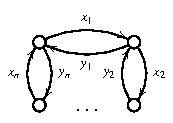
\includegraphics[width=.55\textwidth]{figures/Fig_257_PDF382_Book370.pdf}
    \caption{循环群作用下的箭图（原书 p.370）}
    \label{fig:cyclic-skew-group-quiver}
  \end{figure}
  并满足关系 $x_i y_i-y_{i+1}x_{i+1}=0$。
  \item 计算 $\Pi$ 的 Hochschild 上同调。
  \item 取 $\lambda_i\in(\varepsilon)$，把关系变形为 $x_{i+1}y_{i+1}-y_i x_i=\lambda_i$。证明 $\Pi_\lambda$ 可看成 $\Pi$ 的变形，并确定它的上同调类。
\end{enumerate}
\end{exercise}

\begin{exercise}
计算边界上有 $k$ 个点、内部有 $\ell$ 个标记点的圆盘的拓扑 Fukaya 范畴的 Hochschild 上同调。
\end{exercise}

\begin{exercise}
设 $X$ 是一个簇。用三种方法确定 $D^{\bullet}\mathrm{Coh}\,X$ 的 Hochschild 上同调：
\begin{enumerate}[label=(\roman*)]
  \item 取生成元 $E$，计算 $A_\infty$ 代数
  \[
    E^{\bullet}=\mathrm{Coh}^{\bullet}X(E,E)
  \]
  的 Hochschild 上同调；
  \item 另一种刻画是 $X\times X$ 中对角线结构层的 Ext 环：
  \[
    \mathrm{HH}=\mathrm{Coh}^{\bullet}_{X\times X}(D,D),
  \]
  其中
  \[
    D(U\times V)=\mathcal O(U\times V)/
    \langle f\mid \forall x\in U\cap V,\ f(x,x)=0\rangle;
  \]
  \item Hochschild--Kostant--Rosenberg 定理说明，它也等于多向量场层的整体截面：
  \[
    \mathrm{HH}^i=\Gamma(\wedge^iT).
  \]
\end{enumerate}
证明当 $X=\mathbb P^1$ 时，这三种定义彼此一致。
\end{exercise}

\begin{exercise}
计算 $\mathrm{MF}^{\pm}(\mathbb C^3,XYZ)$ 的 Hochschild 上同调。
\end{exercise}

\begin{exercise}
通过变形轨形范畴
\[
  \mathrm{MF}^{\pm}([\mathbb C^3/G],XYZ),
\]
求出亏格为 $3$ 的曲线的镜像对称，其中 $G=\langle g\mid g^7=1\rangle$，且
\[
  g(X,Y,Z)=\bigl(e^{2\pi i/7}X,e^{4\pi i/7}Y,e^{8\pi i/7}Z\bigr).
\]
\end{exercise}

\begin{exercise}
为例~\ref{ex:pants-filling-genus-one} 中三穿孔环面的 Fukaya 范畴的变形二元乘积所出现的幂级数写出显式表达式。
\end{exercise}

\begin{exercise}
令 $(T,M)$ 为一个单穿孔环面，$L_0,L_1$ 是两条把环面切成正方形、且穿孔点位于正方形中心的曲线。给两条曲线都赋予非平凡自旋结构。在相对 Fukaya 范畴中，$L_0\oplus L_1$ 的自同态环是四维的，由恒等态射和两个态射 $p:L_0\to L_1$、$p^*:L_1\to L_0$ 张成。求
\[
  \mu_3(p,p^*,p)
\]
关于穿孔点变形参数 $\hbar$ 的幂级数（另见\bookcite{162}）。
\end{exercise}

\begin{exercise}
通过变形轨形范畴
\[
  \mathrm{MF}^{\pm}([\mathbb C^3/G],XYZ),
\]
求出亏格为 $1$ 的曲线的镜像对称，其中 $G=\langle g\mid g^4=1\rangle$，且
\[
  g(X,Y,Z)=(iX,iY,-Z).
\]
\end{exercise}

\begin{exercise}
计算 Sklyanin 代数
\[
  S=Skl_{\alpha\beta\gamma}/\langle X,Y,Z\rangle
\]
的简单表示的 Ext--$A_\infty$ 代数。可以假定 $\alpha,\beta,\gamma$ 一般取值，使得
\[
  \operatorname{Ext}^{>3}_{Skl_{\alpha\beta\gamma}}(S,S)=0.
\]
\end{exercise}

\chapterreview{%
\textbf{全章地位。}第 9 章处理带标记（穿孔）曲面，本章处理闭曲面：闭曲面没有可用的弧系，只能靠“变形 + 填充标记点”。技术上以 $A_\infty$ 代数变形理论与 Hochschild 上同调为骨架，几何上以裤子曲面为基本块，最终给出亏格 $g\ge2$ 闭曲面的 Seidel--Efimov 镜像与环面的 Cho--Hong--Lau 镜像函子。这是全书第一次真正把“同调镜像对称”作为定理陈述出来。

\textbf{知识脉络。}Hochschild 上链复形与 Gerstenhaber 括号 $\to$ 一阶变形由 $\mathrm{HH}^1$ 描述、形式变形由 Maurer--Cartan 方程描述、等价类由 $\mathrm{HC}^0$ 的指数作用给出 $\to$ Bardzell 双模分解算出经典上同调 $\to$ HKR 与 Kontsevich 形式性定理把变形翻译成 Poisson 双向量 $\to$ 温和代数的 $\mathrm{HH}^{\bullet}$ 显式计算（绕标记点的 $\ell_m$ 与绕面的 $\ell_f$ 不对称）$\to$ $A_\infty$ 扩张判据认出温和结构 $\to$ 填充标记点后锯齿拉格朗日的自同态环由 $\Lambda_3$ 变形为 $E^\hbar_Z$ $\to$ Koszul 对偶给出 Sklyanin 代数版本 $\to$ 一般框架：镜像函子 $F(X)=(A\otimes\mathcal C(B,X),d)$。

\textbf{核心结论。}（1）$A$ 的一阶变形按等价分类由 $\mathrm{HH}^1(A)$ 描述；形式变形由 $\mathrm{HC}^1(A)\otimes(\hbar)$ 中满足 $dx+\tfrac12[x,x]=0$ 的元素描述，轨道即等价类。（2）HKR 定理：$\mathrm{HH}^{\bullet}_{\mathrm{clas}}(\widehat R)\cong\widehat R\otimes\Lambda^{\bullet}\mathrm{Der}$；Kontsevich 形式性定理把 Maurer--Cartan 方程化为 $[\psi,\psi]=0$，故每个 Poisson 双向量给出一个形式变形。（3）锯齿拉格朗日 $Z$ 的自同态代数 $E_Z^{\pm}\cong\Lambda_3$，而 $\mu(p_x,p_y,p_z)=-\iota$；填三个 $2g+1$ 阶轨形点后 $E^\hbar_Z\cong\Lambda_\gamma$，于是 $D^\pi\mathrm{Fuk}^{\bullet}(S_{abc})\cong_\infty D^\pi\mathrm{MF}^{\pm}(\mathbb C^3,-XYZ+X^{2g+1}+Y^{2g+1}+Z^{2g+1})$。（4）$g=1$ 时乘积是三角数的无穷和，必须取 $\mathbb C[[\hbar]]$ 并在 $\mathbb C((\hbar))$ 上工作，镜像退化为 $XYZ=0$ 的三节点曲线；非交换版本以 $Skl_{\alpha\beta\gamma}/\langle\ell\rangle\cong D^\infty\mathrm{Coh}^{\bullet}E$ 收尾。（5）Koszul 对偶把以顶点为严格单位元的 $A_\infty$ 结构一一对应到 $\widehat{\mathbb C Q}$ 上的 dg 结构，$\mu\mapsto d_\mu$，且 $A_\infty$ 公理等价于 $d_\mu^2=0$。（6）镜像函子由 $dx=\mu(x)+\mu(x,b)+\cdots$ 与 $d^2x=\ell x$ 定义，在双重锯齿一致时猜想为等价。

\textbf{辨析与提醒。}其一，$\mathrm{HC}^{\bullet}$ 用直积而非直和，故 $\ell_f$ 的各次幂可作形式求和、$\ell_m$ 的不行；$\mathrm{HH}^1$ 分母中的 $\ell_i\ell_j\ (i\ne j)$ 正来自这一不对称。其二，$\mathbb Z_2$ 分次下 $\ell_m^r$ 与 $\ell_f^r$ 的 $A_\infty$ 次数都是 $1$，不能按经典次数读它们的幂。其三，$\hbar$ 不可省：$g=1$ 与 $g>1$ 的差别不在几何直觉而在收敛性，$\hbar\to0$ 是奇异极限。其四，镜像函子一般不是等价：标记点周围的小圆与锯齿拉格朗日不相交，因而被消去；只有填充标记点、并且 $Q$ 与 $Q^\vee$ 都锯齿一致时才期望等价。

\textbf{评注。}本章技术密度最高，作者的取舍也最明显：用 Hochschild 上同调把交换与非交换情形塞进同一条等价链，代价是许多计算只给结论（温和代数的 $\mathrm{HH}^{\bullet}$ 用谱序列一笔带过，Orlov 定理直接引用）。这种写法适合有基础的读者按图索骥，初学者则应配合 Efimov 与 Cho--Hong--Lau 的原文补算。值得注意的是，作者把“填充标记点”解释为“消除弦端点造成的阻碍”，这与第 11 章“特殊曲线即半稳定对象”互为表里：稳定化之后 $A$ 侧的对象才是闭的，$B$ 侧才得到真正的 Landau--Ginzburg 模型。全章唯一悬而未决的问题是镜像函子何时为等价，双重锯齿一致仍只是猜想——这也提醒读者，本书给出的是“可算的候选镜像”，而非完整定理。}
